% !TEX root = ../McCoy-Dissertation.tex
\Appendix{On X-ray Spectral Lines}\label{ap:quantum_spectral}
%%%%%%%%%%%%%%%%%%%%%%%%%%%%%%%%%%%%%%%%%--------------------------------------------------
Chemical abundances in the solar photosphere provide an estimate for which atomic nuclei are expected to be the most abundant in the Universe overall as a result of supernovae and other baryon-dispersing processes that have taken place in the Milky Way Galaxy \cite{Rolfs88,Carroll07}. 
The top ten most abundant isotopes inferred from multi-wavelength spectral observations \cite{Grevesse98,Asplund09} are those listed in \cref{tab:astro_element_nuclei_mass}: after hydrogen and helium, the most abundant is element is oxygen followed by carbon, neon, nitrogen, magnesium, silicon, iron and sulfur in decreasing proportions. 
These are the primary atomic nuclei generated by stars with mass $M_{*} \gtrapprox 8 M_{\odot}$. 
\begin{table}[]
 \centering
 \caption[Nuclear masses for stable isotopes of astrophysically abundant elements]{Nuclear masses for stable isotopes of astrophysically abundant elements compared to the mass of the electron, $m_e$ [\emph{cf.\@} \cref{tab:fundamental_constants}]. Data are listed in order of standard solar abundance \cite{Grevesse98,Asplund09}.}\label{tab:astro_element_nuclei_mass}
 \begin{tabular}{@{}lllll@{}} 
 \toprule
 isotope & nucleus & mass \\ \midrule
 hydrogen-1 & 1 proton & $\SI{1.673e-27}{\kilogram} \approx \num{1800} m_e$ \\
 helium-4 & 2 protons + 2 neutrons & $\SI{6.646e-27}{\kilogram} \approx \num{7300} \, m_e$ \\
 \midrule
 oxygen-16 & 8 protons + 8 neutrons & $\SI{2.656e-26}{\kilogram} \approx \num{29200} \, m_e$ \\
 carbon-12 & 6 protons + 6 neutrons &  $\SI{1.993e-26}{\kilogram} \approx \num{21900} \, m_e$ \\
 neon-20 & 10 protons + 10 neutrons & $\SI{3.3209e-26}{\kilogram} \approx \num{36400} \, m_e$ \\
 nitrogen-14 & 7 protons + 7 neutrons & $\SI{2.325e-26}{\kilogram} \approx \num{25500} \, m_e$ \\
 magnesium-24 & 12 protons + 12 neutrons & $\SI{3.983e-26}{\kilogram} \approx \num{43700} \, m_e$ \\
 silicon-28 & 14 protons + 14 neutrons & $\SI{4.646e-26}{\kilogram} \approx \num{51000} \, m_e$ \\
 iron-56 & 26 protons + 30 neutrons & $\SI{9.288e-26}{\kilogram} \approx \num{102000} \, m_e$ & \\
 sulfur-32 & 16 protons + 16 neutrons & $\SI{5.309e-26}{\kilogram} \approx \num{58200} \, m_e$ & \\
 \bottomrule
 \end{tabular}
 \end{table}  
To summarize briefly, following the \emph{main sequence} lifespan of such a massive star, where hydrogen ($\mathcal{Z}=1$) is converted into helium ($\mathcal{Z}=2$) in its core for tens to hundreds of millions of years, the newly-generated helium nuclei (also known as \emph{alpha particles}) through the \emph{triple-alpha} process\footnote{Note that an alpha particle (\emph{i.e.} a helium-4 nucleus) is composed of two protons and two neutrons. In the triple-alpha process, two alpha particles fuse to form the unstable isotope beryllium-8 ($\mathcal{Z}=4$) that then fuses with a third alpha particle to form a stable carbon-12 nucleus.} begin to fuse into nuclei of carbon ($\mathcal{Z}=6$), which in turn fuse further with alpha particles to synthesize nuclei of oxygen ($\mathcal{Z}=8$) and neon ($\mathcal{Z}=10$) \cite{Rolfs88,Carroll07}. 
Due to the sufficiently high core temperature achieved in high-mass stars, carbon nuclei ultimately are able to fuse together to generate more oxygen and neon in addition to sodium and magnesium ($\mathcal{Z}=11,12$). 
As density and temperature increase further, oxygen nuclei also fuse to produce a core consisting mostly of silicon ($\mathcal{Z}=14$) in addition to other byproducts such as magnesium, phosphorous and sulfur ($\mathcal{Z}=12,15,16$). 
Lastly, a series of reactions starting with silicon fusing with helium commences to produce a core dominated by iron ($\mathcal{Z}=26$) prior to the occurrence of a \emph{core-collapse supernova} that ejects these materials into the interstellar medium \cite{Rolfs88,Carroll07,Ryden10}.
During the explosion, other elements with $\mathcal{Z} \lessapprox 26$ are synthesized in relative proportions that depend on the mass of the star, $M_{*}$, as well as other heavier elements in much lower abundances \cite{Woosley86,Rolfs88}. 
Left behind is a neutron star for $M_{*} \lessapprox 25 M_{\odot}$ or a black hole for still more massive stars. 
Meanwhile, the majority of elements heavier than iron are thought to be generated in rare quantities only during extremely energetic events such as the collision of orbiting neutron stars \cite{Kasen17}. 

With the exception of iron due to its relatively high $\mathcal{Z}$, the inner-most electrons (\emph{i.e., K-shell} electrons; see \cref{tab:shell_orbitals}) in the abundant elements listed in \cref{tab:astro_element_nuclei_mass}, save hydrogen and helium, have binding energies characteristic of the soft x-ray spectrum, where photon energy ranges from $\SI{250}{\electronvolt} \lessapprox \mathcal{E}_{\gamma} \lessapprox \SI{2}{\kilo\electronvolt}$. 
Additionally, $\mathcal{E}_e$ for electrons in the next higher-laying shell of iron (\emph{i.e.,} the \emph{L-shell}) fall within this range [\emph{cf.\@} \cref{tab:astro_element_binding}]. 
\begin{table}[]
 \centering
 \caption[Electronic binding energies for the inner-most electrons in neutral atoms of astrophysically abundant elements]{Electronic binding energies, $\mathcal{E}_e$, and associated electromagnetic wavelengths for the inner-most electrons in neutral atoms of the astrophysically abundant elements listed in \cref{tab:astro_element_nuclei_mass}. While the lightest elements are characteristic of vacuum and extreme ultraviolet (UV) radiation, those with $\mathcal{Z} \geq 6$ have K-shell electronic binding energies falling in the soft x-ray and beyond [\emph{cf.\@} \cref{tab:first_element_binding}]. Additionally, L-shell binding energies approach soft x-ray energies for elements heavier than sulfur (not listed are L-shell binding energies for $\mathcal{Z} < 14$) \cite{Attwood17}.}\label{tab:astro_element_binding}
 \begin{tabular}{@{}lllll@{}} 
 \toprule
 chemical element & shell & binding energy & wavelength & spectral band \\ \midrule
 hydrogen ($\mathcal{Z}=1$) & K & \SI{13.6}{\electronvolt} & \SI{91.16}{\nano\metre} & vacuum UV \\
 helium ($\mathcal{Z}=2$) & K & \SI{24.6}{\electronvolt} & \SI{50.4}{\nano\metre} & vacuum UV \\
 \midrule
 oxygen ($\mathcal{Z}=8$) & K & \SI{543.1}{\electronvolt} & \SI{2.28}{\nano\metre} & soft x-ray \\
 carbon ($\mathcal{Z}=6$) & K & \SI{284.2}{\electronvolt} & \SI{4.36}{\nano\metre} & soft x-ray \\
 neon ($\mathcal{Z}=10$) & K & \SI{870.2}{\electronvolt} & \SI{1.42}{\nano\metre} & soft x-ray \\
 nitrogen ($\mathcal{Z}=7$) & K & \SI{409.9}{\electronvolt} & \SI{3.03}{\nano\metre} & soft x-ray \\
 magnesium ($\mathcal{Z}=12$) & K & \SI{1303.0}{\electronvolt} & \SI{0.952}{\nano\metre} & soft x-ray \\ \midrule
 silicon ($\mathcal{Z}=14$) & K & \SI{1838.9}{\electronvolt} & \SI{0.674}{\nano\metre} & soft x-ray \\
 \hspace{5mm}'' \hspace{12mm}'' & L & \SI{149.7}{\electronvolt} & \SI{8.28}{\nano\metre} & extreme UV \\ 
 \hspace{5mm}'' \hspace{12mm}'' & L & \SI{99.8}{\electronvolt} & \SI{12.4}{\nano\metre} & extreme UV \\
 \hspace{5mm}'' \hspace{12mm}'' & L & \SI{99.2}{\electronvolt} & \SI{12.5}{\nano\metre} & extreme UV \\ \midrule
 iron ($\mathcal{Z}=26$) & K & \SI{7112.0}{\electronvolt} & \SI{0.174}{\nano\metre} & x-ray \\ 
 \hspace{3mm}'' \hspace{10mm}'' & L & \SI{844.6}{\electronvolt} & \SI{1.47}{\nano\metre} & soft x-ray \\
 \hspace{3mm}'' \hspace{10mm}'' & L & \SI{719.9}{\electronvolt} & \SI{1.72}{\nano\metre} & soft x-ray \\
 \hspace{3mm}'' \hspace{10mm}'' & L & \SI{706.8}{\electronvolt} & \SI{1.75}{\nano\metre} & soft x-ray \\ \midrule
 sulfur ($\mathcal{Z}=16$) & K & \SI{2472}{\electronvolt} & \SI{0.502}{\nano\metre} & soft x-ray \\
 \hspace{5mm}'' \hspace{11mm}'' & L & \SI{230.9}{\electronvolt} & \SI{5.37}{\nano\metre} & extreme UV \\
 \hspace{5mm}'' \hspace{11mm}'' & L & \SI{163.6}{\electronvolt} & \SI{7.58}{\nano\metre} & extreme UV \\
 \hspace{5mm}'' \hspace{11mm}'' & L & \SI{162.5}{\electronvolt} & \SI{7.63}{\nano\metre} & extreme UV \\
 \bottomrule
 \end{tabular}
 \end{table}
Electrons in these inner-most shells listed in \cref{tab:astro_element_binding} are also the outer-most electrons in highly-charged ions by definition. 
However, the listed data pertain to neutral atoms \cite{Attwood17} whereas K-shell and L-shell electrons in highly-charged ions have binding energies that are somewhat larger due to a lack of outer-shell electrons; this has the consequence that for elements such as silicon and sulfur, L-shell binding energies move into the soft x-ray spectrum as the degree of ionization increases \cite{Kahn02,Paerels03}. 
Therefore, overall, atoms with $6 \leq \mathcal{Z} \lessapprox 14$ ionized down to the K-shell and atoms with $16 \lessapprox \mathcal{Z} \lessapprox 26$ ionized down to the L-shell have their outer-most electrons bound with soft x-ray energies. 
With cosmic abundance weighted toward lower $\mathcal{Z}$, \emph{hydrogen-like} and \emph{helium-like} ions of $6 \leq \mathcal{Z} \lessapprox 14$, where just one or two bound K-shell electrons remain, respectively, are of particular interest for soft x-ray spectroscopy. 
Before prominent spectral lines from these ions are discussed in \cref{sec:selection_rules_hydrogen,sec:selection_rules_helium}, basics of spectral line formation and \emph{electromagnetic-multipole transitions} are outlined in \cref{sec:form_spectral,sec:multipole}, respectively. 
A summary is then given in \cref{sec:apBsummary}. 

\section{Formation of Spectral Lines}\label{sec:form_spectral}
%%%%%%%%%%%%%%%%%%%%%%%%%%%%%%%%%%%%%%--------------------------------------------------
Until \cref{sec:selection_rules_hydrogen,sec:selection_rules_helium}, where details of specific ions are considered, the quantum-mechanical Hamiltonian $\underline{\mathcal{H}}_{\text{atom}}$ defined by \cref{eq:generic_ion_Hamiltonian} is taken to describe a hypothetical two-level atom, where a single electron is subject to an arbitrary force as it makes a jump between two quantum energy levels, and in doing so, interacts with the quantized electromagnetic field to absorb or emit radiation [\emph{cf.\@} \cref{sec:single_absorption_emission}]. 
According to Fermi's golden rule [\emph{cf.\@} \cref{sec:transition_rate_sub}], the probability for such a bound-bound transition to occur increases indefinitely as $\mathscr{P} (t) = \Gamma t$, where $\Gamma$ is given by \cref{eq:transition_rate}. 
While $\Gamma^{-1}$ provides a typical timescale for a certain transition to occur, this does not hold for long timescales because the fact that the probability for an electron to be in its initial state decreases as $t$ progresses must be taken into account \cite{Fontana_82,Griffiths05,kapitell4}. 
If it is assumed that the electron is undergoing a bound-bound transition from some electron-photon state, $\ket{A}$ to another state, $\ket{B}$, the probability of the electron being in the initial state $\ket{A}$ is $1- \mathscr{P} (t)$, where $\mathscr{P} (t) \neq \Gamma t$ is the probability for the transition to occur. 
Then, the rate of change for $\mathscr{P} (t)$ is proportional to the probability of the electron being in state $\ket{A}$:
\begin{subequations}
\begin{equation}
 \dv{\mathscr{P} (t)}{t} = \Gamma \left[ 1- \mathscr{P} (t) \right] .
 \end{equation}
This differential equation can be solved to give 
\begin{equation}\label{eq:probability_decay}
 \mathscr{P} (t) = 1 - \mathrm{e}^{- \Gamma t} ,
 \end{equation}
\end{subequations}
which states that the probability for the transition to have occurred by a time $t$ exhibits asymptotic behavior with $\Gamma$ as a damping parameter. 
Alternatively, this can be argued by considering a distribution of $\mathcal{N}_0$ ions that are all supposed to be in state $\ket{A}$ at some time $t=0$ \cite{Townsend00,kapitell4}. 
The number of ions that remain in state $\ket{A}$ is a function of time, $\mathcal{N}_A (t)$, defined by the following differential equation:
\begin{subequations}
\begin{equation}
 \dv{\mathcal{N}_A (t)}{t} = - \Gamma \mathcal{N}_A (t) ,
 \end{equation}
which can be solved to give $\mathcal{N}_A (t) = \mathcal{N}_0 \mathrm{e}^{- \Gamma t}$. 
Therefore, the probability that $\mathcal{N}_B (t)$ ions have transitioned to state $\ket{B}$ after a time $t$ can be written as  
\begin{equation}\label{eq:number_decay}
 \mathcal{N}_B (t) = \mathcal{N}_0 - \mathcal{N}_A (t) =  \mathcal{N}_0 \left( 1 - \mathrm{e}^{- \Gamma t} \right) ,
 \end{equation}
\end{subequations}
which is equivalent to the probability given by \cref{eq:probability_decay} \cite{Townsend00}. 

In contrast to the \emph{sinc-squared} behavior of first-order transitions [\emph{cf.\@} \cref{fig:sinc_squared}], the decaying transition probability considered here is characteristic of a damped oscillator. 
That is, it is analogous to the spectrum of a classical electromagnetic wave that starts at time $t=0$ and decays over a time interval $\mathcal{T}$, which can be taken to approach infinity \cite{Fontana82}.  
In direct analogy to \cref{eq:wave}, let the magnitude of the electric field for this wave be represented using
\begin{equation}\label{eq:wave_pulse_decay}
    u(t) =
    \begin{cases}
      u_0 \cos \left( \Phi - \omega_0 t \right) \mathrm{e}^{- \frac{1}{2} \Gamma t} , & 0 \leq t \leq \mathcal{T} \\
      0, & \text{otherwise,} 
    \end{cases}
  \end{equation}
where $\omega_0$ effectively plays the role of the transition frequency of a quantum system, $\omega_{\text{trans}} \equiv \Delta \mathcal{E}_e / \hbar$ [\emph{cf.\@} \cref{sec:gen_first_order}]. 
Here, a factor of $1/2$ appears in the exponential so that the intensity of the wave (which is proportional to $\norm{u (t)}^2$) depends on $\mathrm{e}^{- \Gamma t}$; in quantum mechanics, it is the wave function that oscillates at $\omega_{\text{trans}}$ and decays according to $\mathrm{e}^{- \frac{1}{2} \Gamma t}$ so that the transition probability has a $\mathrm{e}^{- \Gamma t}$ dependence \cite{Rybicki86}. 

The temporal Fourier transform of \cref{eq:wave_pulse_decay} is \cite{Fontana82}
\begin{align}
 \begin{split}
 u (\omega) &= \int_{-\infty}^{\infty} u(t) \, \mathrm{e}^{i \omega t} \dd{t} = u_0 \int_0^{\mathcal{T}} \cos \left( \Phi - \omega_0 t \right) \mathrm{e}^{- \frac{1}{2} \Gamma t} \mathrm{e}^{i \omega t} \dd{t} \\
 &= \frac{u_0}{2} \left( \mathrm{e}^{-i \Phi} \frac{1 - \mathrm{e}^{i \left( \omega + \omega_0 \right) \mathcal{T}} \mathrm{e}^{- \frac{1}{2} \Gamma \mathcal{T}}}{\frac{1}{2} \Gamma - i \left( \omega + \omega_0 \right)} + \mathrm{e}^{i \Phi} \frac{1 - \mathrm{e}^{i \left( \omega - \omega_0 \right) \mathcal{T}} \mathrm{e}^{- \frac{1}{2} \Gamma \mathcal{T}}}{\frac{1}{2} \Gamma - i \left( \omega - \omega_0 \right)} \right) 
 \end{split}
 \end{align}
while $\norm{u (t)}^2$ is proportional to the wave intensity. 
Assuming $\mathcal{T} \gg \omega_0^{-1}$ so that the $\omega + \omega_0$ term can be neglected, $\norm{u (t)}^2$ can be written as 
\begin{subequations}
\begin{equation}\label{eq:pulse_intensity}
 \norm{u (\omega)}^2 = \frac{u_0^2 \mathcal{T}^2}{4} \left( \frac{1 + \mathrm{e}^{- \Gamma \mathcal{T}} - 2 \cos \left( \Delta \omega \mathcal{T} \right) \mathrm{e}^{- \frac{1}{2} \Gamma \mathcal{T}}}{\left( \Delta \omega \mathcal{T} \right)^2 + \frac{1}{4} \left( \Gamma \mathcal{T} \right)^2 } \right) 
 \end{equation}
and in the limit that $\mathcal{T} \to \infty$, this becomes
\begin{equation}
 \norm{u (\omega)}^2 = \frac{u_0^2}{4} \left( \frac{1}{\Delta \omega^2 + \frac{1}{4} \Gamma^2} \right) ,
 \end{equation}
which can be normalized\footnote{A normalization coefficient, $\mathcal{A}$, can be determined from
\begin{equation*}
 \mathcal{A} \int_{- \infty}^{\infty} \frac{\dd{\omega}}{\left( \omega - \omega_0 \right)^2 + \frac{1}{4} \Gamma^2} = \mathcal{A} \frac{2 \pi}{\Gamma} = 1, 
 \end{equation*}
where, with $a \equiv \Gamma / 2$:
\begin{equation*}
 \int \frac{\dd{\omega}}{\left( \omega - \omega_0 \right)^2 + a^2} = \frac{\arctan \left( \frac{\omega - \omega_0}{a} \right)}{a} + \text{ a constant} .
 \end{equation*}} 
to yield a \emph{Lorentzian} distribution \cite{Fontana82}:
\begin{equation}\label{eq:normalized_lorentzian}
 \norm{u (\omega)}^2 \to \frac{1}{2 \pi} \left( \frac{\Gamma}{\Delta \omega^2 + \frac{1}{4} \Gamma^2} \right) .
 \end{equation}
\end{subequations}
As mentioned in \cref{sec:gen_first_order}, the quantum analog of $\Delta \omega$ for a bound-bound transition is the difference between the nominal energy associated with the transition and the absorbed or emitted photon energy, $\mathcal{E}_{\gamma} \equiv \hbar \omega$:
\begin{equation*}
 \varpi \equiv \frac{\left( \Delta \mathcal{E}_e - \hbar \omega \right)}{\hbar} = \omega_{\text{trans}} - \omega .
 \end{equation*}
Therefore, the radiation absorbed or emitted by a collection of highly-charged ions undergoing a certain transition with $\omega_{\text{trans}}$ and $\Gamma$ is expected, under ideal conditions, to appear as a Lorentzian distribution with a line profile of the form %proportional to:
\begin{equation}\label{eq:normalized_lorentzian_QM}
 \phi_{\text{nat}} \equiv \frac{1}{2 \pi} \left( \frac{\Gamma}{\left( \omega_{\text{trans}} - \omega \right)^2 + \frac{1}{4} \Gamma^2} \right) .
 \end{equation}
In other words, a \emph{naturally-broadened} spectral line is expected to appear as a Lorentzian distribution if it can be assumed that the ions are virtually stationary and non-interacting; other line profiles are discussed in \cref{sec:astro_plasmas}.

The \emph{full width at half maximum (FWHM)} of such a spectral line is equal to $\Gamma$, which is shown graphically in \cref{fig:lorentzian}. 
\begin{figure}
 \centering
 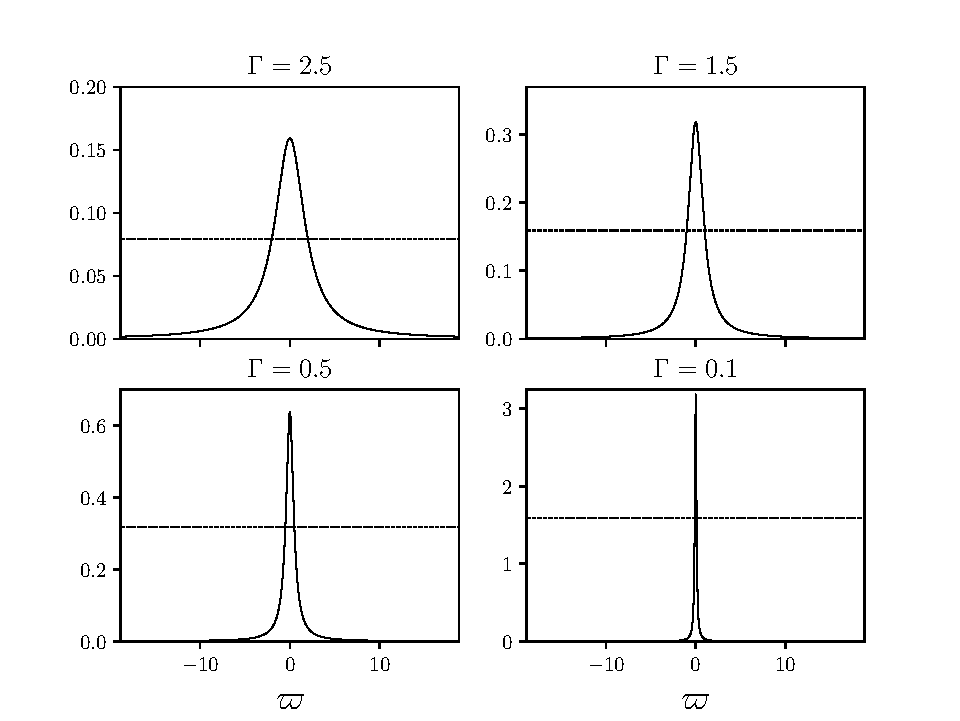
\includegraphics[scale=1]{Appendix-B/Figures/lorentzian_plots.pdf}
 \caption[Plots of Lorentzian functions for naturally-broadened spectral lines]{Plots of Lorentzian functions defined by \cref{eq:normalized_lorentzian_QM} with $\varpi = \omega_{\text{trans}} - \omega$ for four values of the damping term $\Gamma$ using arbitrary units. Dashed lines indicate half maximum with $\text{FWHM}=\Gamma$.}\label{fig:lorentzian}
 \end{figure}
However, this assumes that only the initial state, $\ket{A}$, is broadened, or equivalently, that the electron spends an infinite amount of time in the final state, $\ket{B}$.  
In such a case where this assumption is not justified, $1 / \Gamma_A$ and $1 / \Gamma_B$, the timescales for both states $\ket{A}$ and $\ket{B}$, must be taken into account by making the replacement $\Gamma \to \Gamma_A + \Gamma_B$ \cite{Carroll07,Rybicki86}. 

\section{Electromagnetic-Multipole Transitions}\label{sec:multipole}
%%%%%%%%%%%%%%%%%%%%%%%%%%%%%%%%%%%%%%%%%--------------------------------------------------
In a given species of highly-charged ion, there exist many possible bound states for an inner-shell electron to transition to or from in the process of forming a spectral line [\emph{cf.\@} \cref{sec:form_spectral}]. 
While this depends on how electronic states are populated in a plasma, each of these potential transitions has an associated probabilistic rate, $\Gamma$, that depends on $\norm{\mathcal{M}}^2$ as described by Fermi's golden rule [\emph{cf.\@} \cref{eq:diff_transition_rate,eq:transition_rate}]. 
This transition rate has been formulated in \cref{sec:transition_rate_sub} by first considering the probability for a single transition from one electron-photon state, $\ket{A}$, to another, $\ket{B}$, as a function of time (given by $\norm{\bra{B} \underline{U}_I (t) \ket{A}}^2$) and then integrating this quantity over a range of wave modes. 
To recap, $\underline{U}_I (t)$ is the time-evolution operator from \cref{sec:quantum_perturbations}, given by \cref{eq:first_order_evolution}:
\begin{equation}\label{eq:first_order_evolution_recap}
 \underline{U}_I (t) \approx 1 - \frac{i}{\hbar} \int_0^t \mathrm{e}^{\frac{i}{\hbar} t' \underline{\mathcal{H}}^{(0)}} \underline{\mathcal{H}}^{(1)} \mathrm{e}^{-\frac{i}{\hbar} t' \underline{\mathcal{H}}^{(0)}} \dd{t'} ,
 \end{equation}
where $\underline{\mathcal{H}}^{(0)} = \underline{\mathcal{H}}_{\text{ion}} + \underline{\mathcal{H}}_{\text{EM}}$ is the known Hamiltonian and $\underline{\mathcal{H}}^{(1)}$ is the perturbing Hamiltonian that describes single-photon, bound-bound transitions [\emph{cf.\@} \cref{eq:single_photon_Hamiltonian}]. 
Additionally, \cref{sec:gen_first_order} shows that $\norm{\bra{B} \underline{U}_I (t) \ket{A}}^2$ has a sinc-squared time dependence under first-order perturbation theory, and for a photon state change from $\ket{N_{\mathbold{k},\upsilon}}$ to $\ket{N_{\mathbold{k},\upsilon} - 1}$ or vice-versa, it ends up being proportional to the following, equal quantities [\emph{cf.\@} \cref{eq:abso_stim_matrix_element}] at any given time, $t$:
\begin{subequations}
\begin{align}\label{eq:general_norm_squared_transition}
 \begin{split}
 \text{absorption:} \quad \norm{\mathcal{M}}^2 & = \norm{\bra{\Psi_B} \otimes \bra{\left( N_{\mathbold{k},\upsilon} -1 \right)} \underline{\mathcal{H}}^{(1)} \ket{\Psi_A} \otimes \ket{N_{\mathbold{k},\upsilon}}}^2 \\ 
 \text{emission:} \quad \norm{\mathcal{M}}^2 & = \norm{\bra{\Psi_B} \otimes \bra{N_{\mathbold{k},\upsilon} } \underline{\mathcal{H}}^{(1)} \ket{\Psi_A} \otimes \ket{\left( N_{\mathbold{k},\upsilon} -1 \right) }}^2 .
 \end{split}
 \end{align}
In either case, if $\underline{\mathcal{H}}^{(1)} = (q_e / m_e) \underline{\mathbold{A}} ( \mathbold{r} ) \cdot \underline{\mathbold{p}}$ is inserted and all Fock-space operations are carried out, this quantity reduces to
\begin{equation}\label{eq:general_norm_squared_transition_reduced}
  \norm{\mathcal{M}}^2 = \frac{q_e^2 \hbar N_{\mathbold{k},\upsilon}}{2 m_e^2 \mathcal{V} \epsilon_0 \omega_{\mathbold{k}}} \norm{\hat{\mathbold{e}}_{\mathbold{k},\upsilon} \cdot \bra{\Psi_B} \underline{\mathbold{p}} \mathrm{e}^{\pm i \mathbold{k} \cdot \mathbold{r}} \ket{\Psi_A}}^2 ,
 \end{equation}
\end{subequations}
where $\ket{\Psi_A}$ and $\ket{\Psi_B}$ are the initial and final electron states, respectively, that depend only on the quantum numbers $n$, $\ell$ and $m_{\ell}$ [\emph{cf.\@} \cref{tab:shell_orbitals}] while $\hat{\mathbold{e}}_{\mathbold{k},\upsilon}$ indicates the direction of the photon electric field [\emph{cf.\@} \cref{sec:photon_intro}]. 
Moreover, $-$ in the complex exponential corresponds to emission while $+$ corresponds to absorption. 
Evaluating $\norm{\mathcal{M}}^2$ then gives an indication of the most probable transitions in a particular ion and hence which spectral lines are expected to appear the strongest in a measured spectrum \cite{Kahn02}. 

To motivate the idea that each possible transition in an ion contributes to the spectrum with a certain probability weight, the following classical scenario is considered as a rough analogy. 
The electron states $\ket{\Psi_A}$ and $\ket{\Psi_B}$ describe the spatial probability distributions for the initial and final states of the transitioning electron; these are the so-called \emph{electron clouds} defined by functions of position $\norm{\Psi_A (\mathbold{r})}^2 \equiv \norm{\braket{\mathbold{r}}{\Psi_A}}^2$ and $\norm{\Psi_B (\mathbold{r})}^2 \equiv \norm{\braket{\mathbold{r}}{\Psi_B}}^2$. 
In this analogy, each of these electron clouds described by $\norm{\Psi_{n \ell m} (\mathbold{r})}^2$, which depend on quantum numbers $n$, $\ell$ and $m_{\ell}$, can be thought to represent a continuous distribution of electric charge with a volume density, $\rho(\mathbold{r})$. 
Additionally, the orbital motion of the electron can be thought of as a loop of atomic current so that there is an associated electric current density, $\mathbfcal{J} (\mathbold{r})$, whose vector direction is directly related to $m_{\ell}$. 
From a quantum-mechanical viewpoint, this corresponds to the \emph{probability current} \cite{Griffiths05}:
\begin{equation}
 \mathbfcal{J} (\mathbold{r}) \to \frac{i \hbar}{2 m_e} \left[ \Psi_{n \ell m} (\mathbold{r}) \grad \Psi_{n \ell m}^* (\mathbold{r}) - \Psi_{n \ell m}^* (\mathbold{r}) \grad \Psi_{n \ell m} (\mathbold{r}) \right] \quad \text{with } m \equiv m_{\ell} .
 \end{equation}

As an electron makes a bound-bound-transition from an excited state to the ground state and emits radiation in this classical analogy, these charge and current distributions, $\rho(\mathbold{r},t)$ and $\mathbfcal{J} (\mathbold{r},t)$, oscillate in time between the initial configuration with $\rho_A (\mathbold{r})$ and $\mathbfcal{J}_A (\mathbold{r})$, and the final configuration with $\rho_B (\mathbold{r})$ and $\mathbfcal{J}_B (\mathbold{r})$.\footnote{Note that these two quantities are related to each other through the continuity equation defined by \cref{eq:continuity} \cite{Landau60,Jackson75,Griffiths17,Griffiths05}:
\begin{equation*}
 \div \mathbfcal{J} (\mathbold{r},t) + \pdv{\rho(\mathbold{r},t)}{t} = 0 .
 \end{equation*}}
These oscillating functions, $\rho(\mathbold{r},t)$ and $\mathbfcal{J} (\mathbold{r},t)$, then lead to emission and absorption of electromagnetic waves according to Maxwell's equations [\emph{cf.\@} \cref{sec:EM_waves_vac}]. 
Depending on $\rho (\mathbold{r})$ and $\mathbfcal{J} (\mathbold{r})$ of the initial and final states as well as the frequency of oscillation $(\omega_{\text{trans}} = \Delta \mathcal{E}_e / \hbar$), the radiation pattern associated with such an oscillation may be described as being characteristic of an \emph{electric dipole}, a \emph{magnetic dipole} or more generally, any type of \emph{electromagnetic multipole}, each of which is expected to radiate with a different intensity pattern \cite{Kahn02}. 
The analogy to quantum mechanics is that the probability for a certain transition to occur is related to which type of multipole radiation it is characteristic of. 
There are, however, crucial quantum effects that come into play that weaken this analogy. 
Besides the fact that radiation is discretized into photons, particularly important examples of this include relativistic and spin-related aspects of the electron that are not explained directly by the non-relativistic theory of quantum mechanics.  
While these effects must be taken into account to explain some spectral lines, much of this classical analogy holds for bound-bound radiative processes in highly-charged ions and moreover, different types of transitions are often classified in terms of electromagnetic-multipole radiation [\emph{cf.\@} \cref{sec:allowed_transitions,sec:forbidden_transitions}]. 
Through analyzing these processes, so-called \emph{selection rules} arise that dictate which of these transitions are mostly likely to occur. 

\subsection{Electric-Dipole Transitions}\label{sec:allowed_transitions}
%%%%%%%%%%%%%%%%%%%%%%%%%%%%%%%%%%%%%%%%%--------------------------------------------------
From a classical perspective, the force that an electromagnetic wave exerts on a freely-moving particle at a position $\mathbold{r}$ with charge $-q_e$, mass $m_e$ and velocity $\mathbold{v} \equiv \dv*{\mathbold{r}}{t}$ is the \emph{Lorentz force} \cite{Griffiths17,Jackson75,Rybicki86,Kahn02}:\footnote{This can be shown by carrying out the \emph{Euler-Lagrange equation}:
\begin{equation*} 
\dv{t} \left( \pdv{\mathcal{L} \left( \dot{\mathbold{r}}, \mathbold{r} , t \right)}{\dot{\mathbold{r}}} \right) = \pdv{\mathcal{L} \left( \dot{\mathbold{r}}, \mathbold{r} , t \right)}{\mathbold{r}} ,
 \end{equation*}
where $\mathcal{L} \left( \dot{\mathbold{r}}, \mathbold{r} , t \right)$ is the Lagrangian for a charged particle given by \cref{eq:charged_particle_lagrangian} with $V (r) \to 0$.} 
\begin{align}
\begin{split}\label{eq:Lorentz_force}
 \mathbold{F}(\mathbold{r},\mathbold{v},t) &= - q_e \left( \mathbold{E}(\mathbold{r},t) + \mathbold{v} \times \mathbold{B}(\mathbold{r},t) \right) \\
 &= - q_e \left( \mathbold{E}(\mathbold{r},t) + \frac{\mathbold{v}}{c_0} \times \frac{\mathbold{k}}{k_0} \times \mathbold{E}(\mathbold{r},t) \right) .
 \end{split}
 \end{align}
With the condition $c_0 k_0 \mathbold{B}(\mathbold{r},t) = \mathbold{k} \times \mathbold{E}(\mathbold{r},t)$ for a transverse wave [\emph{cf.\@} \cref{sec:time_harmonic}], the magnetic-field component of the force depends on $\mathbold{v} /c_0$ and hence its magnitude is expected to be small for non-relativistic motion. 
In spirit of the the classical-quantum analogy outlined above, it might then be expected that radiative bound-bound transitions in ions tend to be dominated by the electric-field component, at least in situations where relativistic effects can be neglected. 
Moreover, for bound electrons with small velocities and localized motion, the electric field appears spatially uniform; radiative transitions meeting these criteria should then be characteristic of electric-dipole radiation \cite{deBergevin09}. 
To investigate this, an electric-dipole Hamiltonian term is introduced as the analog to the energy of a classical, point electric dipole: 
\begin{subequations}
\begin{equation}\label{eq:E1_classical}
 U_{\text{E}1} = - \mathbold{\mu}_{\text{E}1} \cdot \mathbold{E}_0 = q_e \mathbold{r} \cdot \mathbold{E}_0 ,
 \end{equation}
where $\mathbold{E}_0$ is a constant electric field. 
Similar to $\underline{\mathcal{H}}^{(1)} = (q_e / m_e) \underline{\mathbold{A}} ( \mathbold{r} ) \cdot \underline{\mathbold{p}}$, this operator is written as 
\begin{equation}\label{eq:E1_hamiltonian}
 \underline{\mathcal{H}}^{(\text{E}1)} \equiv q_e \underline{\mathbold{E}}_0 \cdot \underline{\mathbold{r}} ,
 \end{equation}
where $\underline{\mathbold{E}}_0$ is the electric-field operator defined by \cref{eq:E-field_operator_fixed_linear} with $\mathrm{e}^{\pm i \mathbold{k} \cdot \mathbold{r}} \to 1$ to invoke a constant electric field:
\begin{equation}\label{eq:E-field_operator_fixed_linear_constant}
 \underline{\mathbold{E}}_0 \equiv \sum_{\mathbold{k}} \sum_{\upsilon = 1}^2  i \sqrt{\frac{\hbar \omega_{\mathbold{k}}}{2 \mathcal{V} \epsilon_0}} \hat{\mathbold{e}}_{\mathbold{k},\upsilon} \left[ \underline{a}_{\mathbold{k},\upsilon} - \underline{a}^{\dagger}_{\mathbold{k},\upsilon} \right] ,
 \end{equation}
\end{subequations}
where $\underline{a}_{\mathbold{k},\upsilon}$ and $\underline{a}^{\dagger}_{\mathbold{k},\upsilon}$ are annihilation and creation operators for a Fock state defined by a wave vector $\mathbold{k}$ and a polarization index $\upsilon$ [\emph{cf.\@} \cref{sec:photon_intro}]. 

Noting that bound-bound absorption and emission are opposite processes [\emph{cf.\@} \cref{sec:single_absorption_emission}], the effect that $\underline{\mathcal{H}}^{(\text{E}1)}$ has as a perturbing operator can be examined by considering just one of these cases under the \emph{self-consistent field approximation} [\emph{cf.\@} \cref{sec:atomic_interaction}]. 
To demonstrate this for spontaneous emission, \cref{eq:general_norm_squared_transition} is used to write $\norm{\mathcal{M}}^2$ with $N_{\mathbold{k},\upsilon} = 1$: 
\begin{equation}
 \norm{\mathcal{M}}^2 = \norm{\bra{\Psi_B} \otimes \bra{1_{\mathbold{k},\upsilon} } \underline{\mathcal{H}}^{(1)} \ket{\Psi_A} \otimes \ket{0}}^2 .
 \end{equation}
Inserting $\underline{\mathcal{H}}^{(\text{E}1)}$ [\emph{cf.\@} \cref{eq:E1_hamiltonian}] in place of $\underline{\mathcal{H}}^{(1)}$ gives 
\begin{subequations}
\begin{align}
 \begin{split}
 \norm{\mathcal{M}_{\text{E}1}}^2 &\equiv \norm{\bra{\Psi_B} \otimes \bra{1_{\mathbold{k},\upsilon} } \underline{\mathcal{H}}^{(\text{E}1)} \ket{\Psi_A} \otimes \ket{0}}^2 \\
 &= q_e^2 \norm{\bra{\Psi_B} \otimes \bra{1_{\mathbold{k},\upsilon} } \left( \underline{\mathbold{E}}_0 \cdot \underline{\mathbold{r}} \right) \ket{\Psi_A} \otimes \ket{0}}^2 \\
 &= q_e^2 \frac{\hbar \omega_{\mathbold{k}}}{2 \mathcal{V} \epsilon_0} \norm{\bra{\Psi_B} \left( \hat{\mathbold{e}}_{\mathbold{k},\upsilon} \cdot \underline{\mathbold{r}} \right) \ket{\Psi_A}}^2 , 
 \end{split} 
 \end{align}
while the transition rate, $\Gamma$, is calculated using $\hbar \omega_{\mathbold{k}} = \Delta \mathcal{E}_e$ [\emph{cf.\@} \cref{sec:transition_rate_sub}]: 
\begin{equation}\label{eq:E1_spon_term}
 \norm{\mathcal{M}_{\text{E}1}}^2 \to \frac{q_e^2 \Delta \mathcal{E}_e }{2 \epsilon_0 \mathcal{V}} \norm{\hat{\mathbold{e}}_{\mathbold{k},\upsilon} \cdot \bra{\Psi_B} \underline{\mathbold{r}} \ket{\Psi_A} }^2 .
 \end{equation} 
\end{subequations}
From \cref{eq:emission_matrix_element}, it is known that $\norm{\mathcal{M}}^2$ for a general case of spontaneous emission, using $\underline{\mathcal{H}}^{(1)} = (q_e / m_e) \underline{\mathbold{A}} ( \mathbold{r} ) \cdot \underline{\mathbold{p}}$, is 
\begin{subequations}
\begin{align}
 \begin{split}
 \norm{\mathcal{M}_{\text{spon}} }^2 &\equiv \norm{\bra{\Psi_G} \otimes \bra{1_{\mathbold{k},\upsilon}} \underline{\mathcal{H}}^{(1)} \ket{\Psi_E} \otimes \ket{0}}^2 \\
 &= \frac{q_e^2}{m_e^2} \left( \frac{\hbar}{2 \mathcal{V} \epsilon_0 \omega_{\mathbold{k}}} \right) \norm{\hat{\mathbold{e}}_{\mathbold{k},\upsilon} \cdot \bra{\Psi_G} \underline{\mathbold{p}} \mathrm{e}^{-i \mathbold{k} \cdot \mathbold{r}} \ket{\Psi_E}}^2 ,
 \end{split}
 \end{align}
which, when evaluated at $\hbar \omega_{\mathbold{k}} = \Delta \mathcal{E}_e$ under the approximation $\mathrm{e}^{- i \mathbold{k} \cdot \mathbold{r}} \approx 1$, becomes 
\begin{align}
 \begin{split}\label{eq:normal_spon_term}
 \norm{\mathcal{M}_{\text{spon}} }^2 &\to \norm{\bra{\Psi_G} \otimes \bra{1_{\mathbold{k},\upsilon}} \underline{\mathcal{H}}^{(1)} \ket{\Psi_E} \otimes \ket{0}}^2 \\
 &= \frac{q_e^2}{m_e^2} \left( \frac{\hbar^2}{2 \mathcal{V} \epsilon_0 \Delta \mathcal{E}_e } \right) \norm{\hat{\mathbold{e}}_{\mathbold{k},\upsilon} \cdot \bra{\Psi_G} \underline{\mathbold{p}} \ket{\Psi_E}}^2 .
 \end{split}
 \end{align}
\end{subequations}
Then, using the following quantum operator commutation relation:\footnote{This makes use of the following fundamental commutation relation between the position and momentum operators $\underline{\mathbold{r}}$ and $\underline{\mathbold{p}}$ \cite{Griffiths05,Shankar04}:
\begin{equation}\label{eq:pos_mom_commuation}
 \left[ \underline{r}_{\alpha}, \underline{p}_{\beta} \right] \equiv \underline{r}_{\alpha} \underline{p}_{\beta} - \underline{p}_{\beta} \underline{r}_{\alpha} = i \hbar \delta_{\alpha,\beta} ,
 \end{equation}
where $\alpha, \beta = 1,2,3$ index single components of $\underline{\mathbold{r}}$ and $\underline{\mathbold{p}}$ and $\delta_{\alpha,\beta}$ is a Kronecker delta [\emph{cf.\@} \cref{eq:Kronecker_delta}].}
\begin{subequations}
\begin{equation}
 \left[ \underline{\mathcal{H}}^{(0)} , \underline{\mathbold{r}} \right] \equiv \underline{\mathcal{H}}^{(0)} \underline{\mathbold{r}} - \underline{\mathbold{r}} \underline{\mathcal{H}}^{(0)} = - \frac{i \hbar}{m_e} \underline{\mathbold{p}} , \label{eq:commutation1}
 \end{equation}
where $\underline{\mathcal{H}}^{(0)} = \underline{\mathcal{H}}_{\text{ion}}$ is the unperturbed Hamiltonian, $\norm{\mathcal{M}_{\text{E}1}}^2$ and $\norm{\mathcal{M}_{\text{spon}} }^2$ in \cref{eq:E1_spon_term,eq:normal_spon_term} can be shown to be equivalent by solving \cref{eq:commutation1} for $\underline{\mathbold{p}}$ to write the matrix element in \cref{eq:normal_spon_term} as \cite{Townsend00,Rybicki86} 
\begin{align}\label{eq:dipole_inner_product2}
 \begin{split}
 \hat{\mathbold{e}}_{\mathbold{k},\upsilon} \cdot \matrixel{\Psi_B}{\underline{\mathbold{p}}}{\Psi_A} &= \frac{i m_e}{\hbar} \hat{\mathbold{e}}_{\mathbold{k},\upsilon} \cdot  \left( \matrixel{\Psi_B}{\underline{\mathcal{H}}^{(0)} \underline{\mathbold{r}}}{\Psi_A} - \matrixel{\Psi_B}{\underline{\mathbold{r}} \underline{\mathcal{H}}^{(0)}}{\Psi_A} \right) \\
 &= \frac{i m_e}{\hbar} \underbrace{\left( \mathcal{E}_{B} - \mathcal{E}_{A} \right)}_{\Delta \mathcal{E}_e} \hat{\mathbold{e}}_{\mathbold{k},\upsilon} \cdot \matrixel{\Psi_B}{ \underline{\mathbold{r}} }{\Psi_A} .
 \end{split}
 \end{align}
Carrying out a squared norm on both sides shows that $\norm{\mathcal{M}_{\text{E}1}}^2 = \norm{\mathcal{M}_{\text{spon}} }^2$ under the approximation $\mathrm{e}^{- i \mathbold{k} \cdot \mathbold{r}} \approx 1$ with
\begin{equation}
 \norm{\hat{\mathbold{e}}_{\mathbold{k},\upsilon} \cdot \matrixel{\Psi_B}{\underline{\mathbold{p}}}{\Psi_A}}^2 = \left( \frac{m_e \Delta \mathcal{E}_e}{\hbar} \right)^2 \norm{\hat{\mathbold{e}}_{\mathbold{k},\upsilon} \cdot \matrixel{\Psi_B}{ \underline{\mathbold{r}} }{\Psi_A}}^2 .
 \end{equation}
\end{subequations}

The above analysis indicates that electric-dipole transitions are associated with the $0^{\text{th}}$-order approximation of the complex exponential in \cref{eq:general_norm_squared_transition}, which is valid for either absorption or emission: 
\begin{equation}\label{eq:Taylor_complex_exponential}
 \mathrm{e}^{\pm i \mathbold{k} \cdot \mathbold{r}} = 1 \pm i \mathbold{k} \cdot \mathbold{r} + \frac{\left( \pm i \mathbold{k} \cdot \mathbold{r} \right)^2}{2} \dotsc 
 \end{equation} 
Because a factor of unity enters into $\norm{\mathcal{M}_{\text{E}1}}^2$ in this approximation, these transitions are expected to have relatively large values for the transition rate, $\Gamma$.   
Physically, the condition $\mathbold{k} \cdot \mathbold{r} \ll 1$ implies that the electron undergoing the transition stays localized to within regions much smaller than the wavelength of the absorbed or emitted photon, $\lambda = 2 \pi / k_0 = h c_0 / \mathcal{E}_{\gamma}$  \cite{Shankar04,Townsend00}. 
In other words, the electric field associated with the photon appears spatially uniform to the transitioning electron and this is the case for many transitions in highly-charged ions, or more generally, for transitions involving K-shell electrons in a low-to-mid $\mathcal{Z}$ atom, which have typical radii $\sim a_0 / \mathcal{Z}$ (with $a_0$ as the \emph{Bohr radius}\footnote{This is the distance between the nucleus and the most probable location of a ground-state electron in a hydrogen atom, which can be obtained using the semi-classical \emph{Bohr model of the atom}, where the centripetal force felt by the electron orbiting the proton with a velocity $v$ is balanced by electrostatic attraction between the two charges \cite{Shankar04,Griffiths05}: %\cite{Bohr13a,Bohr13b} ,Tipler07
\begin{equation*}\label{eq:Bohr_model}
 \frac{m_e v^2}{r} = \frac{q_e^2}{4 \pi \epsilon_0 r^2} .
 \end{equation*}
Then, assuming the orbital velocity $v$ takes on only discrete values $v = n \hbar / m_e r$ with $n=1,2,3\dotsc$, the above expression and solving for $r$ with $n=1$ then gives the Bohr radius defined in \cref{tab:fundamental_constants}.}) \cite{Attwood17}. 
For these reasons, $\mathrm{e}^{\pm i \mathbold{k} \cdot \mathbold{r}} \approx 1$ is referred to as the \emph{electric-dipole approximation} and transitions that give $\Gamma \neq 0$ under these conditions tend to be most dominant in a given ion. 

For a transitioning electron, a set of selection rules for the electric-dipole approximation can be determined by first by projecting the electric-dipole matrix element into the position basis:
\begin{equation}
 \hat{\mathbold{e}}_{\mathbold{k},\upsilon} \cdot \bra{\Psi_B} \underline{\mathbold{r}} \ket{\Psi_A} = \hat{\mathbold{e}}_{\mathbold{k},\upsilon} \cdot \int_{-\infty}^{\infty} \Psi_B^* (\mathbold{r}) \, \mathbold{r} \, \Psi_A (\mathbold{r}) \dd[3]{\mathbold{r}} ,
 \end{equation}
and noting that the integral comes out to zero unless the integrand is an even function. 
Because the operator $\underline{\mathbold{r}}$ has \emph{odd parity},\footnote{Broadly, this is defined as the sign change that an operator or wave function incurs from switching the sign on all phase space coordinates: $\underline{\mathbold{p}} \to -\underline{\mathbold{p}}$ and $\underline{\mathbold{r}} \to -\underline{\mathbold{r}}$ \cite{Rybicki86}.} one of the wave functions must be even while the other must be odd to ensure that the integrand is an even function. 
With parity in a one-electron system defined as $(-1)^{\ell}$ (\emph{i.e.}, $+1$ for even and $-1$ for odd), this is verified by \emph{Laporte's rule}, which states that \emph{parity must change during electric-dipole transitions} \cite{Rybicki86,Bethe57}. 
Meanwhile, the spin quantum number, $m_s$, is not expected to change under a pure electric-dipole transition because the \emph{spin-angular-momentum operator}, $\underline{\mathbold{S}}$, does not appear in the perturbing Hamiltonian.
From these considerations, selection rules for an electric-dipole transition between a state with $\ell = \ell_A, m_{\ell} = m_A$ to one with $\ell = \ell_B, m_{\ell} = m_B$ can be stated as 
\begin{align}
 \begin{split}\label{eq:hydrogen_E1_selection_rules}
 \Delta \ell = \ell_B - \ell_A &= \pm 1 \\
 \Delta m_{\ell} = m_B - m_A &= 0, \pm 1 \quad (\text{with } \Delta m_s =0),
  \end{split}
 \end{align}
where the latter follows from the fact that for any given $\ell$, $m_{\ell}$ can take on values $-\ell, -\ell + 1, \dotsc 0, \dotsc \ell -1, \ell$ [\emph{cf.\@} \cref{tab:shell_orbitals}]. 

In a system with two electrons, the parity is given by $(-1)^{\ell_1 + \ell_2}$, where $\ell_{1,2}$ are the azimuthal quantum numbers for each electron. 
Assuming that one electron is in the ground state with $\ell_1 = 0$ while the other is left arbitrary as $\ell_2 = \ell$, the quantum number for the total orbital angular momentum has possible values $L = 0,1$ in the excited state and therefore the selection rules are given by \cite{Rybicki86,Bethe57} 
\begin{align}\label{eq:helium_E1_selection_rules}
 \begin{split}
 \Delta S &= 0 \quad \text{and} \quad \Delta L = 0, \, \pm 1 , \\
 &\text{except for } L = 0 \to L = 0 ,
  \end{split}
 \end{align}
where $\Delta S = 0$ indicates that the total spin of the system does not change in an electric-dipole transition while the $L = 0 \to L = 0$ rules follows from the fact that there must a transfer of angular momentum between the transitioning electron and the interacting photon. 
In any case, the appropriate selection rules dictate which transitions are \emph{allowed} under the electric-dipole approximation while all others are referred to being \emph{forbidden}. 
However, as demonstrated in \cref{sec:forbidden_transitions}, these processes are not truly forbidden but rather occur with much lower probability. 
Electric-dipole transitions can also occur along with a spin magnetic dipole interaction; such a transition is referred to as being \emph{semi-forbidden} and occurs with probability intermediate between allowed and forbidden transitions. 

\subsection{Magnetic-Dipole and Forbidden Transitions}\label{sec:forbidden_transitions}
%%%%%%%%%%%%%%%%%%%%%%%%%%%%%%%%%%%%%%%%%--------------------------------------------------
Bound-bound transitions that yield $\Gamma \neq 0$ under the electric-dipole approximation [\emph{cf.\@} \cref{sec:allowed_transitions}] are expected to occur most frequently and hence contribute to the strongest spectral lines in a given ion, which are also known as \emph{resonance lines}. 
In contrast, transitions that yield $\norm{\mathcal{M}}^2 \neq 0$ only with more terms beyond $\mathrm{e}^{\pm i \mathbold{k} \cdot \mathbold{r}} \approx 1$ are said to be electric-dipole forbidden to indicate their relatively low transition rate, $\Gamma$. 
Based on the arguments given at the start of \cref{sec:allowed_transitions}, magnetic-dipole interactions are expected to be a contributor to these forbidden transitions. 
In analogy to \cref{eq:E1_classical,eq:E1_hamiltonian}, the energy associated with a classical, point magnetic dipole is given by 
\begin{subequations}
\begin{equation}\label{eq:M1_classical}
 U_{\text{M}1} = - \mathbold{\mu}_{\text{M}1} \cdot \mathbold{B}_0 ,
 \end{equation}
where $\mathbold{B}_0$ is a constant magnetic field. 
Then, the corresponding Hamiltonian operator is taken as 
\begin{equation}\label{eq:M1_hamiltonian}
 \underline{\mathcal{H}}^{(\text{M}1)} \equiv - \underline{\mathbold{\mu}}_{\text{M}1} \cdot \underline{\mathbold{B}}_0 ,
 \end{equation}
where $\underline{\mathbold{B}}_0$ is the magnetic-field operator defined in \cref{eq:B-field_operator_fixed_linear} with $\mathrm{e}^{\pm i \mathbold{k} \cdot \mathbold{r}} \to 1$:
\begin{equation}\label{eq:B-field_operator_fixed_linear_constant}
 \underline{\mathbold{B}}_0 = \sum_{\mathbold{k}} \sum_{\upsilon = 1}^2 i \sqrt{\frac{\hbar}{2 \mathcal{V} \epsilon_0 \omega_{\mathbold{k}}}} \mathbold{k} \times \hat{\mathbold{e}}_{\mathbold{k},\upsilon} \left[ \underline{a}_{\mathbold{k},\upsilon} + \underline{a}^{\dagger}_{\mathbold{k},\upsilon} \right] 
 \end{equation}
\end{subequations}
and $\underline{\mathbold{\mu}}_{\text{M}1}$ is the operator for the magnetic-dipole moment. 
This operator includes contributions from both the orbital angular momentum and the intrinsic angular momentum associated with electron spin; these components are considered separately in the following two subsections. 

\subsubsection{Orbital Magnetic-Dipole and Electric-Quadrupole}
%%%%%%%%%%%%%%%%%%%%%%%%%%%%%%%%%%%%%%%%%--------------------------------------------------
In analogy to a classical magnetic dipole, the component of $\underline{\mathbold{\mu}}_{\text{M}1}$ that arises from orbital angular momentum is expressed as \cite{Townsend00,Shankar04,Griffiths05} 
\begin{equation}\label{eq:orbital_moment_operator}
 \underline{\mathbold{\mu}}_{\ell} \equiv - \frac{q_e}{2 m_e} \underline{\mathbold{L}} ,
 \end{equation}
where $\underline{\mathbold{L}}$ is the \emph{orbital-angular-momentum operator}, which is defined as
\begin{subequations} 
\begin{equation}\label{eq:eq:orbit_ang_oper}
 \underline{\mathbold{L}} \equiv \underline{\mathbold{r}} \times \underline{\mathbold{p}} = \hat{\mathbold{x}} \underline{L}_x + \hat{\mathbold{y}} \underline{L}_y + \hat{\mathbold{z}} \underline{L}_z .
 \end{equation}
 Neglecting spin, the quantum numbers $\ell$ and $m_{\ell}$ define eigenvalue relations for $\underline{\mathbold{L}}^2$, as well as for an arbitrary vector component of $\underline{\mathbold{L}}$ to indicate the direction of the magnetic moment. 
Taking this direction to be oriented along the $z$-axis and using the notation $\ket{\Psi_e} \equiv \ket{n, \ell, \, m_{\ell} }$, these relations are \cite{Townsend00,Shankar04,Griffiths05} 
\begin{align}
 \begin{split}\label{eq:orbital_eigenvalues}
 \underline{L}^2 \, \ket{n, \, \ell, \, m_{\ell}} &= \ell (\ell + 1) \hbar^2 \, \ket{n, \, \ell, \, m_{\ell}} \\
 \underline{L}_z \, \ket{n, \, \ell, \, m_{\ell}} &=  m_{\ell} \hbar \, \ket{n, \, \ell, \, m_{\ell}} .
 \end{split}
 \end{align}
Meanwhile, $\underline{L}_x$ and $\underline{L}_y$ can be expressed in terms of $\underline{L}_+$ and $\underline{L}_-$, the raising and lowering operators that serve to change the value of $m_{\ell}$ by $\pm 1$:
\begin{equation}
 \underline{L}_x = \frac{1}{2} \left( \underline{L}_+ + \underline{L}_- \right) \quad \text{and} \quad \underline{L}_y = \frac{i}{2} \left( \underline{L}_- - \underline{L}_+ \right) 
 \end{equation}
with 
\begin{equation}\label{eq:orbital_raise_lower}
 \underline{L}_{\pm} \ket{n, \, \ell, \, m_{\ell}} = \hbar \sqrt{\ell \left( \ell + 1 \right) - m_{\ell} \left( m_{\ell} \pm \right)} \ket{n, \ell, \, \left( m_{\ell} \pm 1 \right)}.
 \end{equation}
\end{subequations}

Defining the orbital-angular-momentum piece of the magnetic-dipole Hamiltonian operator as 
\begin{equation}
 \underline{\mathcal{H}}^{(\text{M}1)}_{\ell} \equiv - \underline{\mathbold{\mu}}_{\ell} \cdot \underline{\mathbold{B}}_0 ,
 \end{equation}
the example of spontaneous emission discussed in \cref{sec:allowed_transitions} is now returned to in order to investigate properties of orbital magnetic-dipole transitions. 
In this situation, the relevant form of $\norm{\mathcal{M}}^2$ with $\underline{\mathcal{H}}^{(\text{M}1)}_{\ell}$ inserted in place of the general expression, $\underline{\mathcal{H}}^{(1)} = (q_e / m_e) \underline{\mathbold{A}} ( \mathbold{r} ) \cdot \underline{\mathbold{p}}$, is 
\begin{align}
 \begin{split}
 \norm{\mathcal{M}_{\text{M}1 \ell}}^2 &\equiv \norm{\bra{\Psi_B} \otimes \bra{1_{\mathbold{k},\upsilon} } \underline{\mathcal{H}}^{(\text{M}1)}_{\ell} \ket{\Psi_A} \otimes \ket{0}}^2 \\
 &= \left( \frac{q_e}{2 m_e} \right)^2 \norm{\bra{\Psi_B} \otimes \bra{1_{\mathbold{k},\upsilon} } \left( \underline{\mathbold{B}}_0 \cdot \underline{\mathbold{L}} \right) \ket{\Psi_A} \otimes \ket{0}}^2 \\
 &= \left( \frac{q_e}{2 m_e} \right)^2 \frac{\hbar}{2 \mathcal{V} \omega_{\mathbold{k}} \epsilon_0} \norm{\bra{\Psi_B} \left[ \left( \mathbold{k} \cross \hat{\mathbold{e}}_{\mathbold{k},\upsilon} \right) \cdot \underline{\mathbold{L}} \right] \ket{\Psi_A}}^2 , 
 \end{split} 
 \end{align}
where it is seen that the perturbing operator takes the form $\left( \mathbold{k} \cross \hat{\mathbold{e}}_{\mathbold{k},\upsilon} \right) \cdot \underline{\mathbold{L}}$. 
As always, this term is evaluated at $\hbar \omega_{\mathbold{k}} = \Delta \mathcal{E}_e$ to arrive at a transition rate given by Fermi's golden rule [\emph{cf.\@} \cref{sec:transition_rate_sub}], where $\Delta \mathcal{E}_e$ is the electronic binding energy difference associated with the transition. 
Then, using the following vector relation \cite{Townsend00}:
\begin{equation}\label{eq:mag_dipole_vector_trick}
 \left( \mathbold{k} \times \hat{\mathbold{e}}_{\mathbold{k},\upsilon} \right) \cdot \underbrace{\left( \underline{\mathbold{r}} \times \underline{\mathbold{p}} \right)}_{\underline{\mathbold{L}}} =  \left( \hat{\mathbold{e}}_{\mathbold{k},\upsilon} \cdot \underline{\mathbold{p}} \right) \left( \mathbold{k} \cdot \underline{\mathbold{r}} \right) - \left( \hat{\mathbold{e}}_{\mathbold{k},\upsilon} \cdot \underline{\mathbold{r}} \right) \left( \mathbold{k} \cdot \underline{\mathbold{p}} \right) ,
 \end{equation}
it can be shown that this magnetic-dipole term appears in $\underline{\mathcal{H}}^{(1)} = (q_e / m_e) \underline{\mathbold{A}} ( \mathbold{r} ) \cdot \underline{\mathbold{p}}$ when the approximation $\mathrm{e}^{\pm i \mathbold{k} \cdot \mathbold{r}} \approx 1 \pm i \mathbold{k} \cdot \mathbold{r}$ is invoked. 
While the first term results in $\bra{\Psi_B} \left( \hat{\mathbold{e}}_{\mathbold{k},\upsilon} \cdot \underline{\mathbold{p}} \right) \ket{\Psi_A}$ for an electric dipole, the next term in the series yields $\bra{\Psi_B} \left( \hat{\mathbold{e}}_{\mathbold{k},\upsilon} \cdot \underline{\mathbold{p}} \right) \left( \mathbold{k} \cdot \underline{\mathbold{r}} \right) \ket{\Psi_A}$, where $\mathbold{r}$ is now treated as the position operator for the electron, $\underline{\mathbold{r}}$. 

By expressing the perturbing operator as 
\begin{align}\label{eq:term_split_trick}
 \begin{split}
 \left( \hat{\mathbold{e}}_{\mathbold{k},\upsilon} \cdot \underline{\mathbold{p}} \right) \left( \mathbold{k} \cdot \underline{\mathbold{r}} \right) &= \frac{1}{2} \underbrace{\left[ \left( \hat{\mathbold{e}}_{\mathbold{k},\upsilon} \cdot \underline{\mathbold{p}} \right) \left( \mathbold{k} \cdot \underline{\mathbold{r}} \right) - \left( \hat{\mathbold{e}}_{\mathbold{k},\upsilon} \cdot \underline{\mathbold{r}} \right) \left( \mathbold{k} \cdot \underline{\mathbold{p}} \right) \right]}_{\text{orbital magnetic dipole}}\\
 &+ \frac{1}{2} \underbrace{ \left[ \left( \hat{\mathbold{e}}_{\mathbold{k},\upsilon} \cdot \underline{\mathbold{p}} \right) \left( \mathbold{k} \cdot \underline{\mathbold{r}} \right) + \left( \hat{\mathbold{e}}_{\mathbold{k},\upsilon} \cdot \underline{\mathbold{r}} \right) \left( \mathbold{k} \cdot \underline{\mathbold{p}} \right) \right] }_{\text{electric quadrupole}},
 \end{split}
 \end{align}
it is seen that terms for both orbital-magnetic-dipole and \emph{electric-quadrupole} transitions are present. 
While the former is evident from \cref{eq:mag_dipole_vector_trick}, the latter term in \cref{eq:term_split_trick} can be recognized as an electric-quadrupole moment by using the following commutation relation:  
\begin{subequations}
\begin{align}
 \begin{split}
 \left[ \underline{\mathcal{H}}^{(0)} , \left( \hat{\mathbold{e}}_{\mathbold{k},\upsilon} \cdot \underline{\mathbold{r}} \right) \left( \mathbold{k} \cdot \underline{\mathbold{r}} \right) \right] &\equiv \underline{\mathcal{H}}^{(0)} \left( \hat{\mathbold{e}}_{\mathbold{k},\upsilon} \cdot \underline{\mathbold{r}} \right) \left( \mathbold{k} \cdot \underline{\mathbold{r}} \right) - \left( \hat{\mathbold{e}}_{\mathbold{k},\upsilon} \cdot \underline{\mathbold{r}} \right) \left( \mathbold{k} \cdot \underline{\mathbold{r}} \right) \underline{\mathcal{H}}^{(0)} \\ 
 &= - \frac{i \hbar }{m_e} \left[ \left( \hat{\mathbold{e}}_{\mathbold{k},\upsilon} \cdot \underline{\mathbold{r}} \right) \left( \mathbold{k} \cdot \underline{\mathbold{p}} \right) + \left( \mathbold{k} \cdot \underline{\mathbold{r}} \right) \left( \hat{\mathbold{e}}_{\mathbold{k},\upsilon} \cdot \underline{\mathbold{p}} \right) \right] ,
 \end{split}
 \end{align}
where $\underline{\mathcal{H}}^{(0)} = \underline{\mathcal{H}}_{\text{ion}}$.\footnote{Motivated by Fitzpatrick \cite{Fitzpatrick_QM}, this result is obtained from carrying out the following operations, where $\hat{\mathbold{e}}$ is shorthand for $\hat{\mathbold{e}}_{\mathbold{k},\upsilon}$:
\begin{align*}
 &\left[ \underline{\mathcal{H}}^{(0)} , \left( \hat{\mathbold{e}} \cdot \underline{\mathbold{r}} \right) \left( \mathbold{k} \cdot \underline{\mathbold{r}} \right) \right] = \sum_{\alpha,\beta} \hat{e}_{\alpha} k_{\beta} \left[ \underline{\mathcal{H}}^{(0)}, \underline{r}_{\alpha} \underline{r}_{\beta} \right] = \sum_{\alpha,\beta} \hat{e}_{\alpha} k_{\beta} \underline{r}_{\alpha} \underbrace{\left[ \underline{\mathcal{H}}^{(0)}, \underline{r}_{\beta} \right]}_{\text{\cref{eq:commutation1}}} + \sum_{\alpha,\beta} \hat{e}_{\alpha} k_{\beta} \underbrace{\left[ \underline{\mathcal{H}}^{(0)}, \underline{r}_{\alpha} \right]}_{\text{\cref{eq:commutation1}}} \underline{r}_{\beta} \\ 
 &\quad = - \frac{i \hbar }{m_e} \sum_{\alpha,\beta} \hat{e}_{\alpha} k_{\beta} \left( r_{\alpha} p_{\beta} + \underbrace{p_{\alpha} r_{\beta}}_{\text{use \cref{eq:pos_mom_commuation}}} \right) = - \frac{i \hbar }{m_e} \sum_{\alpha,\beta} \hat{e}_{\alpha} k_{\beta} \left( r_{\alpha} p_{\beta} + r_{\beta} p_{\alpha} - i \hbar \delta_{\alpha,\beta} \right) \\
 &\quad = - \frac{i \hbar }{m_e} \left[ \left( \hat{\mathbold{e}} \cdot \mathbold{r} \right) \left( \mathbold{k} \cdot \mathbold{p} \right) + \left( \mathbold{k} \cdot \mathbold{r} \right) \left( \hat{\mathbold{e}} \cdot \mathbold{p} \right) - i \hbar \underbrace{\left( \hat{\mathbold{e}} \cdot \mathbold{k} \right)}_0 \right] ,
 \end{align*}
where $\alpha$ and $\beta$ index single components of $\underline{\mathbold{r}}$, $\underline{\mathbold{p}}$, $\mathbold{k}$ and $\hat{\mathbold{e}}$ while $\delta_{\alpha,\beta}$ is a Kronecker delta.} 
Using this relation, the effect that this latter term has as a perturbing operator can be determined through evaluating the following matrix element:
\begin{align}
 \begin{split}
 &\matrixel{\Psi_B}{\left[ \left( \hat{\mathbold{e}}_{\mathbold{k},\upsilon} \cdot \underline{\mathbold{r}} \right) \left( \mathbold{k} \cdot \underline{\mathbold{p}} \right) + \left( \mathbold{k} \cdot \underline{\mathbold{r}} \right) \left( \hat{\mathbold{e}}_{\mathbold{k},\upsilon} \cdot \underline{\mathbold{p}} \right) \right]}{\Psi_A}  \\
 &= \frac{i m_e}{\hbar} \left( \matrixel{\Psi_B}{\underline{\mathcal{H}}^{(0)} \left( \hat{\mathbold{e}}_{\mathbold{k},\upsilon} \cdot \underline{\mathbold{r}} \right) \left( \mathbold{k} \cdot \underline{\mathbold{r}} \right)}{\Psi_A} - \matrixel{\Psi_B}{\left( \hat{\mathbold{e}}_{\mathbold{k},\upsilon} \cdot \underline{\mathbold{r}} \right) \left( \mathbold{k} \cdot \underline{\mathbold{r}} \right) \underline{\mathcal{H}}^{(0)}}{\Psi_A} \right) \\
 &= \frac{i m_e}{\hbar} \underbrace{\left( \mathcal{E}_{B} - \mathcal{E}_{A} \right)}_{\Delta \mathcal{E}_e} \matrixel{\Psi_B}{\underbrace{\left( \hat{\mathbold{e}}_{\mathbold{k},\upsilon} \cdot \underline{\mathbold{r}} \right) \left( \mathbold{k} \cdot \underline{\mathbold{r}} \right)}_{\text{electric quadrupole}}}{\Psi_A} ,
 \end{split}
 \end{align}
\end{subequations}
where as in \cref{eq:dipole_inner_product2}, $\Delta \mathcal{E}_e$ is the difference in electronic binding energies for the initial and final states. 
With $\alpha,\beta =1,2,3$ indexing tensor components, the energy associated with a classical electric quadrupole is 
\begin{subequations}
\begin{equation}\label{eq:electric_quad_energy}
 \frac{1}{6} \sum_{\alpha,\beta} \mathcal{Q}_{\alpha,\beta} \pdv{E_{\beta}}{r_{\alpha}} ,
 \end{equation}
with being $\mathcal{Q}_{\alpha,\beta}$ the \emph{quadrupole-moment tensor} \cite{Jackson75}.
For a set of point charges with $-q_e$, this can be written as 
\begin{equation}\label{eq:electric_quad_moment}
 \mathcal{Q}_{\alpha,\beta} = -q_e \left( 3 r_{\alpha} r_{\beta} - r^2 \delta_{\alpha,\beta} \right) .
 \end{equation}
\end{subequations}

With the approximation $\mathrm{e}^{\pm i \mathbold{k} \cdot \mathbold{r}} \approx 1 \pm i \mathbold{k} \cdot \mathbold{r}$, the spatial derivative of the electric field with a vector direction $\hat{e}_{\beta}$ gives $k_{\alpha} \hat{e}_{\beta}$ so that \cref{eq:electric_quad_energy} becomes 
\begin{subequations}
\begin{equation}\label{eq:electric_quad_energy_approx}
 \frac{1}{6} \sum_{\alpha,\beta} \mathcal{Q}_{\alpha,\beta} k_{\alpha} \hat{e}_{\beta} . 
 \end{equation}
Then, it can be shown using \cref{eq:electric_quad_energy,eq:electric_quad_moment} that the term $\left(\hat{\mathbold{e}} \cdot \mathbold{r} \right) \left( \mathbold{k} \cdot \mathbold{r} \right)$ is proportional to the energy of an electric quadrupole:
\begin{equation}
 \sum_{\alpha,\beta} \mathcal{Q}_{\alpha,\beta} k_{\alpha} \hat{e}_{\beta} \propto \sum_{\alpha,\beta} \left( 3 r_{\alpha} r_{\beta} \hat{e}_{\beta} - r^2 \delta_{\alpha,\beta} k_{\alpha} \hat{e}_{\beta} \right) = \left( 3 \hat{\mathbold{e}} \cdot \mathbold{r} \right) \left( \mathbold{k} \cdot \mathbold{r} \right) - r^2 \underbrace{\mathbold{k} \cdot \hat{\mathbold{e}}}_0 . 
 \end{equation}
\end{subequations}
This indicates that, unlike an electric-dipole transition, an electric-quadrupole transition is subject to a photon electric field that varies spatially to a small degree. 
Like an electric-dipole transition, however, such a transition does not depend on angular momentum and hence there should be no effect on electron spin. 
Ultimately, the relevant matrix element depends on the square of the position operator, $\underline{\mathbold{r}}^2$, instead of $\underline{\mathbold{r}}$ as it does in \cref{eq:dipole_inner_product2} for the case of electric-dipole transitions. 

Because orbital magnetic-dipole transitions depends on the operator $\underline{\mathbold{L}}$ and electric-quadrupole transitions depends on $\underline{\mathbold{r}}^2$, both are associated with even parity. 
This implies that the initial and final wave function in a one-electron system must have the same parity, $(-1)^{\ell}$. 
In the magnetic-dipole case, $\underline{\mathbold{L}}$ can at most change $m_{\ell}$ by one due to the presence of $\mathbold{L}_{\pm}$ [\emph{cf.\@} \cref{eq:orbital_raise_lower}] to first order, while in any case, $\ell$ remains unchanged. 
Therefore, selection rules for such a transition (neglecting spin) can be taken as
\begin{align}
 \begin{split}\label{eq:hydrogen_M1_selection_rules}
 \Delta \ell = \ell_B - \ell_A &= 0 \\
 \Delta m_{\ell} = m_B - m_A &= 0, \pm 1 .
  \end{split}
 \end{align}
For electric-quadrupole transitions, $\ell$ can either stay the same or change by $\pm 2$ to provide even parity overall and thus these selection rules are 
\begin{align}
 \begin{split}\label{eq:hydrogen_E2_selection_rules}
 \Delta \ell = \ell_B - \ell_A &= 0, \pm 2 \\
 \Delta m_{\ell} = m_B - m_A &= 0, \pm 1, \pm 2 ,
  \end{split}
 \end{align}
where it is assumed that there is no change in the spin quantum number, $m_s$. 
Either of these situations can be generalized to two-electron systems, where in particular, it holds true that \emph{the configuration does not change} for magnetic-dipole transitions \cite{Rybicki86}. 
Explained next, this condition can also be fulfilled in the event that the total spin of the system changes while the orbital angular momentum is unaffected. 

\subsubsection{Spin Magnetic-Dipole and Semi-Forbidden}
%%%%%%%%%%%%%%%%%%%%%%%%%%%%%%%%%%%%%%%%%--------------------------------------------------
So far in this appendix, non-relativistic quantum mechanics has been employed and therefore electron spin has not been properly taken into account. 
Because of this, a second component to $\underline{\mathbold{\mu}}_{\text{M}1}$ that depends on electron spin must be added to the perturbing Hamiltonian manually to describe certain phenomena. 
With the total operator written as $\underline{\mathbold{\mu}}_{\text{M}1} \equiv \underline{\mathbold{\mu}}_{\ell} + \underline{\mathbold{\mu}}_{s}$, the spin term is defined as
\begin{subequations}
\begin{equation}\label{eq:spin_moment_operator}
 \underline{\mathbold{\mu}}_{s} \equiv - \frac{q_e g_e}{2 m_e} \underline{\mathbold{S}} ,
 \end{equation} 
where $g_e \approx \num{2.002319}$ is the \emph{g-factor} of electron that arises in relativistic quantum mechanics and 
\begin{equation}\label{eq:spin_ang_oper}
 \underline{\mathbold{S}} = \hat{\mathbold{x}} \underline{S}_x + \hat{\mathbold{y}} \underline{S}_y + \hat{\mathbold{z}} \underline{S}_z
 \end{equation}
is the spin-angular-momentum operator that acts on electron spin states represented by \emph{spinors} of the form $\ket{\chi_e} \equiv \ket{s, \, m_s}$ \cite{Shankar04,Townsend00}. 
In the case of a single electron, $s=1/2$ while $m_s = \pm 1/2$ but more generally, $s$ is the total spin of the system and $m_s$ takes on values $-s, -s + 1, \dotsc 0, \dotsc s -1, s$ that indicate the net spin direction of the system. 
Just as in \cref{eq:orbital_eigenvalues} for orbital angular momentum, the following eigenvalue relations hold: 
\begin{align}
 \begin{split}\label{eq:spin_eigenvalues}
 \underline{S}^2 \, \ket{s, \, m_{s}} &= s (s + 1) \hbar^2 \, \ket{s, \, m_{s}} \\
 \underline{S}_z \, \ket{s, \, m_{s}} &=  m_{s} \hbar \, \ket{s, \, m_{s}} ,
 \end{split}
 \end{align}
while $\underline{S}_x$ and $\underline{S}_y$ can be expressed in terms of $\underline{S}_+$ and $\underline{S}_-$, the raising and lowering operators for spin states that change the value of $m_s$ by $\pm 1$:
\begin{equation}
 %\begin{split}
 \underline{S}_x = \frac{1}{2} \left( \underline{S}_+ + \underline{S}_- \right) \quad \text{and} \quad \underline{S}_y = \frac{i}{2} \left( \underline{S}_- - \underline{S}_+ \right)
 %\end{split}
 \end{equation}
with 
\begin{equation}
 \underline{S}_{\pm} \ket{s, \, m_s} = \hbar \sqrt{\ell \left( \ell + 1 \right) - m_{\ell} \left( m_{\ell} \pm \right)} \ket{s, \, \left( m_s \pm 1 \right)}.
 \end{equation}
\end{subequations}
Considering this piece of the Hamiltonian alone for a one-electron system:
\begin{equation}
 \underline{\mathcal{H}}^{(\text{M}1)}_{s} \equiv - \underline{\mathbold{\mu}}_{s} \cdot \underline{\mathbold{B}}_0 ,
 \end{equation}
it is expected that like in the case of an orbital magnetic-dipole transition, only the direction of the angular momentum, $m_s$, is affected while $s$ cannot change due to parity considerations. 
On the other hand, parity can change if the electric-dipole term $\underline{\mathcal{H}}^{(\text{E}1)} = q_e \underline{\mathbold{B}}_0 \cdot \underline{\mathbold{r}}$ is included with the perturbing Hamiltonian. %from \cref{sec:allowed_transitions}
In this case, the selection rules defined in \cref{eq:hydrogen_E1_selection_rules,eq:helium_E1_selection_rules} are still satisfied but with the added flexibility that the total spin of the system can change by one quantum number. 
Such a \emph{semi-forbidden} transition that requires both electric-dipole and spin-magnetic-dipole interaction is said to produce \emph{intercombination lines}. 

\section{Hydrogen-like Ions}\label{sec:selection_rules_hydrogen}
%%%%%%%%%%%%%%%%%%%%%%%%%%%%%%%%%%%%%%%%%--------------------------------------------------
The single electron bound in a hydrogen-like ion is subject to a central potential established by the nuclear charge, $\mathcal{Z} q_e$. 
In non-relativistic quantum mechanics, where spin is neglected, this is described with the following Hamiltonian operator \cite{Bethe57,Townsend00,Kahn02,Shankar04}: 
\begin{equation}\label{eq:hydrogen_ion_Hamiltonian}
 \underline{\mathcal{H}}_{\text{H}} = \frac{\underline{\mathbold{p}}^2}{2 m_R} - \hbar c_0 \alpha_f \frac{\mathcal{Z}}{\abs{\underline{\mathbold{r}}}} ,
 \end{equation}
where $\alpha_f$ is the fine-structure constant, $\underline{\mathbold{p}}$ and $\underline{\mathbold{r}}$ are the momentum and position operators for the electron and $m_R$ is the two-body reduced mass:
\begin{equation}\label{eq:reduced_mass}
 m_R \equiv \frac{m_e \, m_{\text{nucleus}}}{m_e + m_{\text{nucleus}}} \approx m_{\text{nucleus}}
 \end{equation}
with $m_{\text{nucleus}}$ provided in \cref{tab:astro_element_nuclei_mass} for various astrophysically abundant elements. 
\begin{subequations}
Without spin, wave functions $\braket{\mathbold{r}}{\Psi_e} \equiv \Psi_{n \ell m} (\mathbold{r})$ only depends on $n$, $\ell$ and $m_{\ell}$; they are solutions to the time-independent Schr\"ondiger equation, which can written in spherical coordinates as \cite{Townsend00,Shankar04,Griffiths05} 
\begin{equation}\label{eq:TI_Schrodinger_hydrogen}
 - \left( \frac{\hbar^2}{2 m_R} \laplacian + \hbar c_0 \alpha_f \frac{\mathcal{Z}}{r} \right) \Psi_{n \ell m} (r, \theta, \phi) = \mathcal{E}_{n \ell m} \Psi_{n \ell m} (r, \theta, \phi) \quad \text{with } m \equiv m_{\ell},
 \end{equation}
where the momentum operator takes on the form $\underline{\mathbold{p}} = - i \hbar \grad$ in the position basis and the eigenvalue $\mathcal{E}_{n \ell m}$ is the binding energy of the electron. 
Solutions to \cref{eq:TI_Schrodinger_hydrogen} exist in closed form, where the eigenvalues depend only on the principal quantum number, $n$ \cite{Townsend00,Shankar04,Griffiths05}:
\begin{align}\label{eq:simple_hydrogen_energy_Z}
 \begin{split}
 \mathcal{E}_{n \ell m} \to \mathcal{E}_n &= - \frac{1}{2} m_R c_0^2 \alpha^2_f \frac{\mathcal{Z}^2}{n^2} \\
 \text{with ground state} \quad \mathcal{E}_1 &= - \frac{1}{2} m_R c_0^2 \alpha^2_f \mathcal{Z}^2 \approx \left( \SI{-13.61}{\electronvolt} \right) \mathcal{Z}^2.
 \end{split}
 \end{align}
\end{subequations}

Due to the central-potential symmetry of $\underline{\mathcal{H}}_{\text{H}}$ [\emph{cf.\@} \cref{eq:hydrogen_ion_Hamiltonian}], the eigenfunctions can be split into radial and angular parts \cite{Townsend00,Bethe57,Kahn02,Shankar04}: 
%\begin{subequations} 
\begin{equation}\label{eq:separable_wave_function} 
 \Psi_{n \ell m} (r, \theta, \phi) \equiv \mathcal{R}_{n \ell}(r) \, Y_{\ell m} (\theta,\phi) \quad \text{with } m \equiv m_{\ell}. 
 \end{equation}
Defining $a_R \equiv m_e a_0 / m_R$, the radial component can be written explicitly as
\begin{subequations} 
\begin{equation}\label{eq:radial_solution_Schrodinger}
 \mathcal{R}_{n \ell}(r) = \sqrt{\left( \frac{2 \mathcal{Z}}{n a_R} \right)^3 \frac{(n - \ell -1)!}{2 n \left[ (n + \ell)! \right]^3}} \, \mathrm{e}^{- \mathcal{Z} r / n a_R} \left( \frac{2 \mathcal{Z} r}{n a_R} \right)^{\ell + 1} \mathcal{L}_{n-\ell-1}^{2 \ell + 1} \left( \frac{2 \mathcal{Z} r}{n a_R} \right) 
 \end{equation}  
with 
\begin{equation}\label{eq:radial_solution_Schrodinger_polynomial1}
 \mathcal{L}_{n-\ell-1}^{2 \ell + 1} ( X ) \equiv (-1)^{2 \ell + 1} \left( \dv{X} \right)^{2 \ell + 1} \mathcal{L}_{n-\ell-1} ( X ) ,
 \end{equation}
as an \emph{associated Laguerre polynomial} and 
\begin{equation}\label{eq:radial_solution_Schrodinger_polynomial2}
 \mathcal{L}_{n-\ell-1} ( X ) \equiv \mathrm{e}^{X} \left( \dv{X} \right)^{n-\ell-1} \left( \mathrm{e}^{-X} X^{n-\ell-1} \right) . 
 \end{equation}
\end{subequations}
as a \emph{Laguerre polynomial} of order $n-\ell-1$ \cite{Griffiths05,Shankar04}. 
%\footnote{Defining $X \equiv 2 \mathcal{Z} r / n a_R$, $\mathcal{L}_{n-\ell-1}^{2 \ell + 1} ( X )$ is an \emph{associated Laguerre polynomial}: 
%\begin{equation*}\label{eq:radial_solution_Schrodinger_polynomial1}
% \mathcal{L}_{n-\ell-1}^{2 \ell + 1} ( X ) \equiv (-1)^{2 \ell + 1} \left( \dv{X} \right)^{2 \ell + 1} \mathcal{L}_{n-\ell-1} ( X ) ,
% \end{equation*}
%where $\mathcal{L}_{n-\ell-1} ( X )$ is a \emph{Laguerre polynomial} of order $n-\ell-1$: 
%\begin{equation*}\label{eq:radial_solution_Schrodinger_polynomial2}
% \mathcal{L}_{n-\ell-1} ( X ) \equiv \mathrm{e}^{X} \left( \dv{X} \right)^{n-\ell-1} \left( \mathrm{e}^{-X} X^{n-\ell-1} \right) . 
% \end{equation*} } 
The angular component can be defined in terms of \emph{spherical harmonics}, which form a complete set of orthogonal functions on a unit sphere: 
\begin{subequations}
\begin{equation}\label{eq:angular_solution_Schrodinger}
 Y_{\ell m} (\theta,\phi) = \sqrt{\frac{2 \ell + 1}{4 \pi} \frac{(\ell - m)!}{(\ell + m)!}} \, P_{\ell}^{m} \left[ \cos (\theta) \right] \mathrm{e}^{i m \phi} \quad \text{with } m \equiv m_{\ell} ,
 \end{equation}
where 
\begin{equation}\label{eq:angular_solution_Schrodinger_polynomial1}
 P_{\ell}^{m} \left( X \right) \equiv \left( 1 - X^2 \right)^{|m|/2}  \left( \dv{X} \right)^{|m|} P_{\ell} \left( X \right) 
 \end{equation}
is an \emph{associated Legendre function} with $P_{\ell} \left( X \right)$ being a \emph{Legendre polynomial} given by the \emph{Rodrigues formula} \cite{Griffiths05,Shankar04}: 
\begin{equation}\label{eq:angular_solution_Schrodinger_polynomial2}
 P_{\ell} \left( X \right) \equiv \frac{1}{2^{\ell} \ell !} \left( \dv{X} \right)^{\ell} \left( X^2 - 1 \right)^{\ell} . 
 \end{equation}
\end{subequations}
The eigenfunctions of a hydrogen-like atom constructed under this framework thus are known exactly and can be expressed analytically. 

%\footnote{Defining $X \equiv \cos (\theta) $, $P_{\ell}^{m} \left( X \right)$ is an \emph{associated Legendre function} defined by: 
%\begin{equation*}\label{eq:angular_solution_Schrodinger_polynomial1}
% P_{\ell}^{m} \left( X \right) \equiv \left( 1 - X^2 \right)^{|m|/2}  \left( \dv{X} \right)^{|m|} P_{\ell} \left( X \right) ,
% \end{equation*}
%with $P_{\ell} \left( X \right)$ being a \emph{Legendre polynomial} given by the \emph{Rodrigues formula}: 
%\begin{equation*}\label{eq:angular_solution_Schrodinger_polynomial2}
% P_{\ell} \left( X \right) \equiv \frac{1}{2^{\ell} \ell !} \left( \dv{X} \right)^{\ell} \left( X^2 - 1 \right)^{\ell} . 
% \end{equation*} }

%which form a complete set of orthogonal functions on a unit sphere. 
%\end{subequations}

\subsection{Fine-Structure Corrections}
%%%%%%%%%%%%%%%%%%%%%%%%%%%%%%%%%%%%%%%%%--------------------------------------------------
Together, the functions $\mathcal{R}_{n \ell}(r)$ and $Y_{\ell m} (\theta,\phi)$ [\emph{cf.\@} \cref{eq:radial_solution_Schrodinger,eq:angular_solution_Schrodinger}] effectively describe the shape of an electron cloud given by the probability distribution, $\norm{\Psi_{n \ell m} (r, \theta, \phi)}^2$. 
Additionally, $\mathcal{E}_n$ given by \cref{eq:simple_hydrogen_energy_Z} can be used to arrive at approximate values for centroids of spectral lines that arise from transitioning atomic electrons. 
For example, using $\mathcal{E}_n$ to evaluate the difference in electronic binding energies:
\begin{equation}\label{eq:approx_lyman}
 \Delta \mathcal{E}_e = \mathcal{E}_2 - \mathcal{E}_1 = \frac{3}{8} m_R c_0^2 \alpha^2_f \mathcal{Z}^2 ,
 \end{equation}
shows that transitions between the K-shell and the L-shell fall comfortably within the soft x-ray range for abundant hydrogen-like ions with $6 \lessapprox \mathcal{Z} \lessapprox 14$ [\emph{cf.\@} \cref{tab:astro_element_lyman_approx}].  
\begin{table}[]
 \centering
 \caption[Nominal photon energies for Lyman-alpha transitions in abundant hydrogen-like ions]{Nominal photon energies and associated electromagnetic wavelengths for $n=1$ to $n=2$ transitions in abundant hydrogen-like ions according to non-relativistic quantum mechanics using \cref{eq:approx_lyman}.}\label{tab:astro_element_lyman_approx}
 \begin{tabular}{@{}lllll@{}} 
 \toprule
 chemical element & ion & transition energy & wavelength & spectral band \\ \midrule
 hydrogen ($\mathcal{Z}=1$) & \ion{H}{i} & \SI{10.2}{\electronvolt} & \SI{121.4}{\nano\metre} & far/vacuum UV \\
 helium ($\mathcal{Z}=2$) & \ion{He}{ii} & \SI{40.8}{\electronvolt} & \SI{30.4}{\nano\metre} & extreme UV \\
 oxygen ($\mathcal{Z}=8$) & \ion{O}{viii} & \SI{653.4}{\electronvolt} & \SI{1.90}{\nano\metre} & soft x-ray \\
 carbon ($\mathcal{Z}=6$) & \ion{C}{vi} & \SI{367.5}{\electronvolt} & \SI{3.37}{\nano\metre} & soft x-ray \\
 neon ($\mathcal{Z}=10$) & \ion{Ne}{x} & \SI{1021.0}{\electronvolt} & \SI{1.21}{\nano\metre} & soft x-ray \\
 nitrogen ($\mathcal{Z}=7$) & \ion{N}{vii} & \SI{500.3}{\electronvolt} & \SI{2.48}{\nano\metre} & soft x-ray \\
 magnesium ($\mathcal{Z}=12$) & \ion{Mg}{xii} & \SI{1470.2}{\electronvolt} & \SI{0.843}{\nano\metre} & soft x-ray \\
 silicon ($\mathcal{Z}=14$) & \ion{Si}{xiv} & \SI{2001.1}{\electronvolt} & \SI{0.620}{\nano\metre} & soft x-ray \\
 iron ($\mathcal{Z}=26$) & \ion{Fe}{xxvi} & \SI{6901.7}{\electronvolt} & \SI{0.180}{\nano\metre} & x-ray \\
 \bottomrule
 \end{tabular}
 \end{table}
However, there are relativistic and fermionic effects of the electron that have not been accounted for with non-relativistic treatment of 
quantum mechanics but nonetheless have an effect on electronic binding energies and, therefore, spectral line centroids \cite{Bethe57,Kahn02}. 
While this is more accurately described by relativistic quantum mechanics using the \emph{Dirac equation} or techniques in \emph{quantum field theory}, perturbative corrections to $\underline{\mathcal{H}}_{\text{H}}$ can be introduced to arrive at a corrected expression for electronic binding energy \cite{Griffiths05,Townsend00}: 
\begin{subequations}
\begin{equation}\label{eq:rel_corrections}
 \left( \underline{\mathcal{H}}_{\text{H}} + \text{corrections} \right) \ket{\Psi_e} = \mathcal{E}_{\text{corrected}} \ket{\Psi_e} .
 \end{equation}
In particular, these corrections include higher-order terms to relativistic kinetic energy:
\begin{equation}\label{eq:rel_kinetic_expansion}
 \sqrt{ \underline{\mathbold{p}}^2 c_0^2 + m_e^2 c_0^4} - m_e c_0^2 = \frac{\underline{\mathbold{p}}^2}{2 m_e} - \frac{\underline{\mathbold{p}}^4}{8 m_e^3 c_0^2} + \cdots
 \end{equation}
as well as the \emph{spin-orbit interaction} \cite{Griffiths05,Shankar04}. 
This latter correction arises from the fact that in the reference frame of a bound electron with orbital angular momentum, there is a magnetic field generated by the apparent motion of the nucleus that exerts a force on the spin-magnetic moment; the perturbing Hamiltonian for this interaction is given by 
\begin{equation}\label{eq:spin-orbit}
 \underline{\mathcal{H}}_{\text{S-O}} = \frac{\mathcal{Z} q_e^2}{2 m_e^2 c_0^2 \underline{\mathbold{r}}^3} \, \underline{\mathbold{L}} \cdot \underline{\mathbold{S}} ,
 \end{equation} 
\end{subequations}
which involves the orbital and spin-angular-momentum operators, $\underline{\mathbold{L}}$ and $\underline{\mathbold{S}}$ given by \cref{eq:eq:orbit_ang_oper,eq:spin_ang_oper} \cite{Townsend00}. 

\subsection{Lyman Doublet Splitting}
%%%%%%%%%%%%%%%%%%%%%%%%%%%%%%%%%%%%%%%%%--------------------------------------------------
Taking into account the fine-structure effects described by \cref{eq:rel_corrections,eq:rel_kinetic_expansion,eq:spin-orbit}, the result is that the full expression for electronic binding energy depends on $n$ but also the quantum number for total angular momentum, $j$ \cite{Griffiths05,Townsend00}:
\begin{align}\label{eq:fine_hydrogen_energy_Z}
 \begin{split}
 \mathcal{E}_{\text{corrected}} \to \mathcal{E}_{n,j} &= - \frac{1}{2} m_R c_0^2 \alpha^2_f \frac{\mathcal{Z}^2}{n^2} \left[ 1 + \frac{\alpha_f^2}{n^2} \left( \frac{n}{j + 1/2} - \frac{3}{4} \right) \right] \\
 \text{with ground state} \quad \mathcal{E}_{1,1/2} &= - \frac{1}{2} m_R c_0^2 \alpha^2_f \left( 1 + \frac{1}{4} \alpha_f^2 \right) \mathcal{Z}^2 . 
 \end{split}
 \end{align}
With the electron-spin number being $s = 1/2$, the number $j$ can take on values $\left( \ell + 1/2 \right), \, \left( \ell - 1/2 \right), \, \left( \ell -3/2 \right), \, \ldots, \, \abs{\ell - 1/2}$: in a state with $n=2$ and $\ell = 1$, for example, $j$ can either be $3/2$ or $1/2$ and hence there are two possible transitions to the ground state with $n=1$, $\ell=0$ and $j = 1/2$. 
These can be written in \emph{spectroscopic notation} as \cite{Rybicki86}
\begin{align}\label{eq:hydrogen_doublet}
 \begin{split}
 2 p \; {}^2 \! P_{3/2} &\leftrightarrow 1 s \; {}^2 \! S_{1/2} \quad \text{(resonance)} \\ 
 2 p \; {}^2 \! P_{1/2} &\leftrightarrow 1 s \; {}^2 \! S_{1/2} \quad \text{(intercombination)}.
 \end{split}
 \end{align}
The former transition satisfies the selection rules for a pure electric-dipole transition [\emph{cf.\@} \cref{eq:hydrogen_E1_selection_rules}], where $\Delta \ell =1$ so that $j$ transitions in between $3/2$ and $1/2$. 
In contrast, the latter transition also involves $\Delta \ell =1$ but additionally, the fact that $j$ is unchanged implies that a spin flip must occur. 
With a spin violation to the usual selection rules, this means that this latter transition is semi-forbidden under the electric-dipole approximation [\emph{cf.\@} \cref{sec:allowed_transitions}]. 

These transitions described by \cref{eq:hydrogen_doublet} give rise to resonance and intercombination lines that are revealed to be closely spaced when \cref{eq:fine_hydrogen_energy_Z} is used to calculate $\Delta \mathcal{E}_e$:
\begin{subequations}
\begin{align}
 \text{resonance: } \Delta \mathcal{E}_R &\equiv \mathcal{E}_{2,3/2} - \mathcal{E}_{1,1/2} = \frac{3}{8} m_R c_0^2 \alpha^2_f \left( 1 + \frac{5}{16} \alpha_f^2 \right) \mathcal{Z}^2  \\ 
 \text{intercombination: } \Delta \mathcal{E}_I &\equiv \mathcal{E}_{2,1/2} - \mathcal{E}_{1,1/2} = \frac{3}{8} m_R c_0^2 \alpha^2_f \left( 1 + \frac{11}{48} \alpha_f^2 \right) \mathcal{Z}^2 , 
 \end{align}
where the difference between the two is
\begin{equation}
 \Delta \mathcal{E}_R - \Delta \mathcal{E}_I = \frac{1}{32} m_R c_0^2 \alpha^2_f \mathcal{Z}^2 \approx \left( \SI{0.85}{\electronvolt} \right) \mathcal{Z}^2 ,
 \end{equation}
\end{subequations}
which shows that the resonance transition has a slightly higher energy than the intercombination line. 
Whether or not this doublet of spectral lines are resolved, these \emph{Lyman-alpha} transitions between the K-shell and the L-shell are among the most prominent spectral lines for hydrogen-like ions \cite{Kahn02}. 
Similar Lyman-series transitions exist for other shells with $n > 2$ and $\ell > 1$ but only some values of $j$ obey the electric-dipole selection rules.  
In pure magnetic-dipole transitions, only $m_{\ell}$ or $m_s$ are affected while there cannot be a change in $\ell$. 
Therefore, an electron involved in such a forbidden transition is confined to a single shell so that by \cref{eq:fine_hydrogen_energy_Z}, $\Delta \mathcal{E}_e$ is much smaller than $\mathcal{E}_{\gamma}$ for soft x-rays. % and hence not directly relevant to x-ray spectroscopy.   
An example of an electric-quadrupole transition is a jump between ($n=3$, $\ell=2$) to ($n=1$, $\ell=0$) but such processes have very low transition rates and hence contribute little to measured spectra \cite{Townsend00}. 

\section{Helium-like Ions}\label{sec:selection_rules_helium}
%%%%%%%%%%%%%%%%%%%%%%%%%%%%%%%%%%%%%%%%%--------------------------------------------------
In a helium-like ion, a transitioning electron feels attraction from the central nuclear charge but additionally, it is subject to repulsive force from the second bound electron. 
While important spin-related effects come into play, a non-relativistic Hamiltonian that neglects spin can be written as \cite{Griffiths05,Townsend00,Bethe57,Kahn02} 
\begin{subequations}
\begin{equation}\label{eq:helium_ion_Hamiltonian}
 \underline{\mathcal{H}}_{\text{He}} = \frac{1}{2 m_e} \left( \underline{\mathbold{p}}_1^2 + \underline{\mathbold{p}}_2^2 \right) - \hbar c_0 \alpha_f \left( \frac{\mathcal{Z}}{ \abs{ \underline{ \mathbold{r} }_1 } } + \frac{\mathcal{Z}}{  \abs{ \underline{ \mathbold{r} }_2 } }  - \frac{1}{\abs{ \underline{\mathbold{r}}_2 -  \underline{ \mathbold{r} }_1  }} \right) ,
 \end{equation}
where subscripts$_{1,2}$ indicate the phase-space operators, $\underline{\mathbold{p}}$ and $\underline{\mathbold{r}}$, that act on the wave vectors $\ket{\Psi_{e1}}_1$ and $\ket{\Psi_{e2}}_2$ for each electron.\footnote{These wave vectors can be projected into their respective position bases:
\begin{equation*}
 \braket{\mathbold{r}_1}{\Psi_{e1}}_1 = \Psi_{e1} (\mathbold{r}_1) \quad \text{and} \quad \braket{\mathbold{r}_2}{\Psi_{e2}}_2 = \Psi_{e2} (\mathbold{r}_2) .
 \end{equation*}
With the coordinates interchanged, this is written as 
\begin{equation*}
 \braket{\mathbold{r}_1}{\Psi_{e2}}_1 = \Psi_{e2} (\mathbold{r}_1) \quad \text{and} \quad \braket{\mathbold{r}_2}{\Psi_{e1}}_2 = \Psi_{e1} (\mathbold{r}_2) .
 \end{equation*}
} 
Here, the nucleus is treated as being stationary for simplicity so that the reduced-mass term with $m_R$ [\emph{cf.\@} \cref{eq:reduced_mass}] is omitted. 
Although the Schr\"ondiger equation cannot be solved exactly for $\underline{\mathcal{H}}_{\text{He}}$, approximate solutions can be found by treating the electron-electron repulsion term as a perturbation to two hydrogen-like Hamiltonians for each electron given by \cref{eq:hydrogen_ion_Hamiltonian} with $m_R = m_e$:
\begin{equation}\label{eq:helium_ion_Hamiltonian2}
 \underline{\mathcal{H}}_{\text{He}} = \underline{\mathcal{H}}_{\text{H}1} + \underline{\mathcal{H}}_{\text{H}2} + \frac{\hbar c_0 \alpha_f}{\abs{ \underline{\mathbold{r}}_2 -  \underline{ \mathbold{r} }_1 }} .
 \end{equation}
\end{subequations}

Separately, the two electrons in a helium-like ion have quantum numbers $n_{1,2}$, $\ell_{1,2}$ and $m_{\ell \, 1,2}$ but as discussed in \cref{sec:allowed_transitions}, it is assumed that at least one of the electrons is in the ground state so that $n_1 = 1, \, \ell_1 = 1 \text{ and } m_{\ell \, 1} = 0$ while the other is left arbitrary with $n_2 \to n, \, \ell_2 \to \ell \text{ and } m_{\ell \, 2} \to m_{\ell}$. 
However, with two overlapping electron wave vectors, \emph{identical-particle} and spin effects must also be taken into account to determine how the electrons exist in superposition with a combined wave function $\Psi_e \left( \mathbold{r}_1, \mathbold{r}_2 \right)$. 
These phenomena hinge on the rules of \emph{Fermi-Dirac statistics}, which require that the overall state of the system be antisymmetric under exchange of particle coordinates \cite{Shankar04,Griffiths05}. 
This overall state includes the combined wave vector $\ket{\Psi_e}$ as well as a spinor $\ket{\chi_e} \equiv \ket{S, \, m_S}$ that describes the total spin of the system. 

\subsection{The Ground State}\label{sec:helium_ground}
%%%%%%%%%%%%%%%%%%%%%%%%%%%%%%%%%%%%%%%%%--------------------------------------------------
In the ground state of a helium-like ion with $n = 1, \, \ell = 0 \text{ and } m_{\ell} = 0$ for both $\ket{\Psi_{e1}}_1$ and $\ket{\Psi_{e2}}_2$, the \emph{Pauli exclusion principle} \cite{Shankar04,Griffiths05} dictates that the two electrons must have opposite spin such that the total spin quantum number is $S=0$ and the configuration is written in spectroscopic notation as
\begin{equation}
 1 s^2 \; {}^1 \! S_{0} .
 \end{equation}
Using the following shorthand for spin-up and spin-down states $\ket{s, \, m_s}$ of the individual electrons: 
\begin{align}
\begin{split}
  \ket{1/2, \, +1/2}_1 &\equiv \ket{\uparrow}_1 \quad \ket{1/2, \, +1/2}_2 \equiv \ket{\uparrow}_2 \\
 \ket{1/2, \, -1/2}_1 &\equiv \ket{\downarrow}_1 \quad \ket{1/2, \, -1/2}_2 \equiv \ket{\downarrow}_2 , 
 \end{split}
 \end{align}
the total spinor $\ket{\chi_e}$ is an antisymmetric \emph{singlet state} \cite{Griffiths05,Townsend00}:
\begin{subequations}
\begin{equation}
 \ket{0, \, 0} = \frac{1}{\sqrt{2}} \left[ \ket{\uparrow}_1 \otimes \ket{\downarrow}_2 - \ket{\downarrow}_1 \otimes \ket{\uparrow}_2 \right] .
 \end{equation}
This allows the wave vector to be a symmetric superposition of $\ket{\Psi_{e1}}$ and $\ket{\Psi_{e2}}$ known as \emph{parahelium}:
\begin{align}
 \begin{split}
 \ket{\Psi_e} &= \frac{1}{\sqrt{2}} \left[ \ket{\Psi_{e1}}_1 \otimes \ket{\Psi_{e2}}_2 + \ket{\Psi_{e2}}_1 \otimes \ket{\Psi_{e1}}_2 \right] \\
 \text{or} \quad \Psi_e ( \mathbold{r}_1, \mathbold{r}_2 ) &= \frac{1}{\sqrt{2}} \left[ \Psi_{e1} (\mathbold{r}_1) \, \Psi_{e2} (\mathbold{r}_2) + \Psi_{e2} (\mathbold{r}_1) \, \Psi_{e1} (\mathbold{r}_2) \right] .
 \end{split}
 \end{align} 
In the special case of the ground-state configuration, both electrons have identical quantum numbers so this is written as $\ket{1, \, 0, \, 0}_1 \otimes \ket{1, \, 0, \, 0}_2$ using $\ket{n, \, \ell, \, m_{\ell}}$ for a single-electron state. 
The overall state that combines the symmetric wave vector and the antisymmetric spinor then is written as 
\begin{equation}
 \ket{1 s^2 \; {}^1 \! S_{0}} \equiv \ket{1, \, 0, \, 0}_1 \otimes \ket{1, \, 0, \, 0}_2 \otimes \ket{0, \, 0} .
 \end{equation}
\end{subequations}

In principle, the total energy of the ground state is determined from the following expectation value:
\begin{subequations}
\begin{align}
 \begin{split}
 \mathcal{E}_{(1 s^2 \; {}^1 \! S_{0})} &\equiv \expval{ \underbrace{ \underline{\mathcal{H}}_{\text{He}} }_{ \text{ \cref{eq:helium_ion_Hamiltonian2} } } }{1 s^2 \; {}^1 \! S_{0}} \\
 &= \underbrace{ \expval{\underline{\mathcal{H}}_{\text{H}1}}{1 s^2 \; {}^1 \! S_{0}} }_{\mathcal{E}_1} + \underbrace{\expval{\underline{\mathcal{H}}_{\text{H}2}}{1 s^2 \; {}^1 \! S_{0}}}_{\mathcal{E}_1} \\ 
 &\quad \quad+ \underbrace{\expval{ \left( \frac{\hbar c_0 \alpha_f}{\abs{ \mathbold{r}_2 - \mathbold{r}_1 }} \right) }{1 s^2 \; {}^1 \! S_{0}} }_{\text{electron-electron}} ,
 \end{split}
 \end{align}
where $\mathcal{E}_1 = - \frac{1}{2} m_e c_0^2 \alpha^2_f \mathcal{Z}^2$ is the ground-state energy of a hydrogen-like ion\footnote{Neglecting spin and relativistic effects, $\mathcal{E}_1$ is given by \cref{eq:simple_hydrogen_energy_Z} with $n=1$ and $m_R = m_e$.} while the last term is the energy contributed by the electron-electron repulsion. %[chapter 12]
Following Townsend~\cite{Townsend00}, this piece of the expectation value can be evaluated in the position basis using the following matrix element:\footnote{Note that because $\underline{\mathcal{H}}_{\text{He}}$ does not depend on the spin operator, $\underline{\mathbold{S}}$, 
\begin{equation*}
 \expval{ \underline{\mathcal{H}}_{\text{He}} }{1 s^2 \; {}^1 \! S_{0}} = \bra{1, \, 0, \, 0}_1 \otimes \bra{1, \, 0, \, 0}_2 \underline{\mathcal{H}}_{\text{He}} \ket{1, \, 0, \, 0}_1 \otimes \ket{1, \, 0, \, 0}_2 \underbrace{ \braket{0, \, 0} }_1 .
 \end{equation*}} 
\begin{align}\label{eq:perturbing_helium_term}
 \begin{split}
 &\expval{ \left( \frac{\hbar c_0 \alpha_f}{\abs{ \underline{\mathbold{r}}_2 -  \underline{ \mathbold{r} }_1 }} \right) }{1 s^2 \; {}^1 \! S_{0}} \\
 &\quad \quad \quad \quad = \iint \underbrace{\norm{\braket{\mathbold{r}_1}{1, \, 0, \, 0}_1}^2}_{\norm{\Psi_e (\mathbold{r}_1)}^2} \underbrace{\norm{\braket{\mathbold{r}_2}{1, \, 0, \, 0}_2}^2}_{\norm{\Psi_e (\mathbold{r}_2)}^2}  \left( \frac{\hbar c_0 \alpha_f}{\abs{ \underline{\mathbold{r}}_2 -  \underline{ \mathbold{r} }_1 }} \right) \dd[3]{\mathbold{r}_1} \dd[3]{\mathbold{r}_2}   .
 \end{split}
 \end{align}
\end{subequations} 
For both sets of coordinates, $\mathbold{r}_1$ and $\mathbold{r}_2$, the wave function takes the form of a hydrogen-like ion as in \cref{eq:separable_wave_function,eq:radial_solution_Schrodinger,eq:angular_solution_Schrodinger}:
\begin{equation}
 \braket{\mathbold{r}}{n, \, \ell, \, m } = \Psi_e (\mathbold{r}) = \mathcal{R}_{n \ell}(r) \, Y_{\ell m} (\theta,\phi) \quad \text{with } m \equiv m_{\ell} ,
 \end{equation}
where in the case of the ground state, 
\begin{equation}
 \braket{\mathbold{r}}{1, \, 0, \, 0 } = \mathcal{R}_{1 0}(r) \, Y_{0 0} (\theta,\phi) = \frac{1}{\sqrt{\pi}} \left( \frac{\mathcal{Z}}{a_0} \right)^{3/2} \mathrm{e}^{-\frac{\mathcal{Z}}{a_0} r} .
 \end{equation}
\begin{subequations}
While the mathematics are not carried here, the integral in \cref{eq:perturbing_helium_term} comes out to \cite{Townsend00} %by Townsend~\cite{Townsend00}
\begin{equation} %\footnote{See \cite[chapter 7]{Griffiths05} and \cite[chapter 12]{Townsend00}.}
 \expval{ \left( \frac{\hbar c_0 \alpha_f}{\abs{ \underline{\mathbold{r}}_2 -  \underline{ \mathbold{r} }_1 }} \right) }{1 s^2 \; {}^1 \! S_{0}} = \frac{5}{8} m_e c_0^2 \alpha_f^2 \mathcal{Z} \approx \left( \SI{34}{\electronvolt} \right) \mathcal{Z} 
 \end{equation}
and the total energy of the ground state then is %according to this then is 
\begin{equation}
 \mathcal{E}_{(1 s^2 \; {}^1 \! S_{0})} = \underbrace{- m_e c_0^2 \alpha^2_f \mathcal{Z}^2}_{2 \mathcal{E}_1} + \frac{5}{8} m_e c_0^2 \alpha_f^2 \mathcal{Z} = m_e c_0^2 \alpha_f^2 \mathcal{Z} \left( \frac{5}{8} - \mathcal{Z} \right) .
 \end{equation}
\end{subequations} 
However, this approximation is several percentage points off from the experimentally-determined value. 
%cannot be solved exactly. 
A more accurate result for the ground state energy comes from the \emph{variational method}, where the wave function for each electron has an effective value for $\mathcal{Z}$ that is allowed to vary; this is written as $\tilde{\mathcal{Z}}$ so that the modified wave function for both sets of coordinates is \cite{Griffiths05,Townsend00}
\begin{subequations}
\begin{equation}
 \tilde{\Psi}_e (\mathbold{r}) = \frac{1}{\sqrt{\pi}} \left( \frac{\tilde{\mathcal{Z}}}{a_0} \right)^{3/2} \mathrm{e}^{-\frac{ \tilde{\mathcal{Z}}}{a_0} r} .
 \end{equation}
By expressing the Hamiltonian in \cref{eq:helium_ion_Hamiltonian} as
\begin{align}\label{eq:helium_ion_Hamiltonian_variational}
 \begin{split}
 \underline{\mathcal{H}}_{\text{He}} &= \frac{1}{2 m_e} \left( \underline{\mathbold{p}}_1^2 + \underline{\mathbold{p}}_2^2 \right) - \hbar c_0 \alpha_f \left( \frac{ \tilde{\mathcal{Z}}}{ \abs{ \underline{ \mathbold{r} }_1 } } + \frac{ \tilde{\mathcal{Z}}}{  \abs{ \underline{ \mathbold{r} }_2 } } \right)  \\
 &\quad + \hbar c_0 \alpha_f \left( \frac{ \left( \tilde{\mathcal{Z}} - \mathcal{Z} \right)}{ \abs{ \underline{ \mathbold{r} }_1 } } + \frac{ \left( \tilde{\mathcal{Z}} - \mathcal{Z} \right) }{ \abs{ \underline{ \mathbold{r} }_2 } } + \frac{1}{\abs{ \underline{\mathbold{r}}_2 -  \underline{ \mathbold{r} }_1 }} \right) 
 \end{split}
 \end{align}
and then carrying out the expectation value $\expval{\underline{\mathcal{H}}_{\text{He}}}{1 s^2 \; {}^1 \! S_{0}}$ gives a function of $\tilde{\mathcal{Z}}$ that minimizes at $\tilde{\mathcal{Z}} = \mathcal{Z} - \frac{5}{16}$ so that 
\begin{equation}
 \mathcal{E}_{(1 s^2 \; {}^1 \! S_{0})} \approx \underbrace{- m_e c_0^2 \alpha^2_f}_{\SI{-27.2}{\electronvolt}} \left( \mathcal{Z} - \frac{5}{16}  \right)^2 .
 \end{equation}
\end{subequations}
This result yields $\mathcal{E}_{(1 s^2 \; {}^1 \! S_{0})} = \SI{-77.5}{\electronvolt}$ for $\mathcal{Z} = 2$ whereas the most accepted experimentally-determined value is $\mathcal{E}_{(1 s^2 \; {}^1 \! S_{0})} = \SI{-79.0}{\electronvolt}$ \cite{Griffiths05,Townsend00}.\footnote{Note that this binding energy lays in the extreme UV spectrum while analogous binding energies for helium-like ions of low-to-mid $\mathcal{Z}$ exist in the soft x-ray spectrum.} 

\subsection{L-shell Excited States and Prominent Transitions}\label{eq:helium_Lshell}
%%%%%%%%%%%%%%%%%%%%%%%%%%%%%%%%%%%%%%%%%--------------------------------------------------
In contrast to the ground state of helium [\emph{cf.\@} \cref{sec:helium_ground}], the total electronic spin can be either $S=0$ or $S=1$ if one of the two bound electrons is in an excited state, in which case there are three possible \emph{triplet states}, $\ket{1, \, m_S}$, that give the same total spin \cite{Griffiths05,Townsend00}: 
\begin{subequations}
\begin{align}
 \begin{split}
 \ket{1, \, +1} = \ket{\uparrow}_1 \otimes \ket{\uparrow}_2, \quad \ket{1, \, -1} = \ket{\downarrow}_1 \otimes \ket{\downarrow}_2 \\
 \text{and} \quad \ket{1, \, 0} = \frac{1}{\sqrt{2}} \left( \ket{\uparrow}_1 \otimes \ket{\downarrow}_2 + \ket{\downarrow}_1 \otimes \ket{\uparrow}_2 \right) .
 \end{split}
 \end{align}
Because each of these spinors are symmetric with respect to particle exchange, the spatial part of the overall wave vector then must be antisymmetric to satisfy Fermi-Dirac statistics: 
\begin{align}
 \begin{split}
 \ket{\Psi_e} &= \frac{1}{\sqrt{2}} \left[ \ket{\Psi_{e1}}_1 \otimes \ket{\Psi_{e2}}_2 - \ket{\Psi_{e2}}_1 \otimes \ket{\Psi_{e1}}_2 \right] \\
 \text{or} \quad \Psi_e ( \mathbold{r}_1, \mathbold{r}_2 ) &= \frac{1}{\sqrt{2}} \left[ \Psi_{e1} (\mathbold{r}_1) \, \Psi_{e2} (\mathbold{r}_2) - \Psi_{e2} (\mathbold{r}_1) \, \Psi_{e1} (\mathbold{r}_2) \right] ;
 \end{split}
 \end{align}
this is referred to as \emph{orthohelium} \cite{Griffiths05,Townsend00}. 
\end{subequations}
While the ground state of a helium-like ion is necessarily parahelium, configurations where one electron is an excited state can either be parahelium or orthohelium. 

Despite the fact that spin does not appear in $\underline{\mathcal{H}}_{\text{He}}$ [\emph{cf.\@} \cref{eq:helium_ion_Hamiltonian}], parahelium and orthohelium tend to have different electronic binding energies that arise from identical-particle and spin effects that have no clear classical analog. 
In particular, with the wave vector being symmetric in parahelium, the spatial part of the system exhibits boson-like properties such that electrons tend to be closer together than they do in orthohelium, where the antisymmetric nature of the wave vector causes the opposite phenomenon \cite{Griffiths05,Townsend00}. 
Because of this, electrons in parahelium experience slightly more repulsion from each other and hence are expected to have higher energy (\emph{i.e.}, binding energy that is less negative) than electrons in orthohelium.  
This breaks degeneracy in the spin configuration and therefore it is useful to consider each possible state with $S=0$ and $S=1$ as being a contributor to measured spectral lines. 
For example, if $n=2$ and $S=0$ in an excited parahelium state, the total angular momentum is either $J=1$ or $J=0$ depending on if the excited electron is associated with $\ell=1$ or $\ell=0$. 
These two configurations can be written in spectroscopic notation as
\begin{subequations}
\begin{equation}\label{eq:he_singlets}
 1s \, 2 p \; {}^1 \! P_{1} \quad \text{and} \quad 1s \, 2 s \; {}^1 \! S_{0} ,
 \end{equation}
with the following wave vectors:
\begin{align}
 \ket{1s \, 2 p \; {}^1 \! P_{1} } &= \frac{1}{\sqrt{2}} \left[ \ket{1, \, 0, \, 0}_1 \otimes \ket{2, \, 1, \, m_{\ell}}_2 + \ket{2, \, 1, \, m_{\ell}}_1 \otimes \ket{1, \, 0, \, 0}_2 \right] \otimes \ket{0, \, 0} \\
 \ket{1s \, 2 s \; {}^1 \! S_{0} } &= \frac{1}{\sqrt{2}} \left[ \ket{1, \, 0, \, 0}_1 \otimes \ket{2, \, 0, \, 0 }_2 + \ket{2, \, 0, \, 0 }_1 \otimes \ket{1, \, 0, \, 0}_2 \right] \otimes \ket{0, \, 0} .
 \end{align}
\end{subequations}
%\begin{subequations}
For $n=2$ and $S=1$, as another example, the total angular momentum takes on values $J=2,1,0$ from the addition of $L=\ell$ and $S$. 
If $\ell = 0$, it must be that $J=1$ and the configuration is
\begin{subequations}
\begin{equation}\label{eq:he_triplet1}
 1s \, 2 s \; {}^3 \! S_{1} 
 \end{equation}
with 
\begin{equation}
 \ket{1s \, 2 s \; {}^3 \! S_{1}} = \frac{1}{\sqrt{2}} \left[ \ket{1, \, 0, \, 0}_1 \otimes \ket{2, \, 0, \, 0 }_2 - \ket{2, \, 0, \, 0 }_1 \otimes \ket{1, \, 0, \, 0}_2 \right] \otimes \ket{1, \, m_S} .
 \end{equation}
\end{subequations}
In the event that $\ell = 1$, all three possible values of $J$ are possible: 
\begin{subequations}
\begin{equation}\label{eq:he_triplet2}
 1s \, 2 s \; {}^3 \! P_{2} , \quad 1s \, 2 s \; {}^3 \! P_{1} \quad \text{and} \quad 1s \, 2 s \; {}^3 \! P_{0} ,
 \end{equation}
%\end{subequations}
with
\begin{align}
\begin{split}
 \ket{1s \, 2 s \; {}^3 \! P_{2}} &= \frac{1}{\sqrt{2}} \left[ \ket{1, \, 0, \, 0}_1 \otimes \ket{2, \, 1, \, \pm 2}_2 - \ket{2, \, 1, \, \pm 2}_1 \otimes \ket{1, \, 0, \, 0}_2 \right] \otimes \ket{1, \, \pm 2} \\
 \ket{1s \, 2 s \; {}^3 \! P_{1}} &= \frac{1}{\sqrt{2}} \left[ \ket{1, \, 0, \, 0}_1 \otimes \ket{2, \, 1, \, 0}_2 - \ket{2, \, 1, \, 0}_1 \otimes \ket{1, \, 0, \, 0}_2 \right] \otimes \ket{1, \, \pm 1} \\
 \ket{1s \, 2 s \; {}^3 \! P_{0}} &= \frac{1}{\sqrt{2}} \left[ \ket{1, \, 0, \, 0}_1 \otimes \ket{2, \, 1, \, \mp 1}_2 - \ket{2, \, 1, \, \mp 1}_1 \otimes \ket{1, \, 0, \, 0}_2 \right] \otimes \ket{1, \, \pm 1} .
 \end{split}
 \end{align}
\end{subequations}
%and $\mathcal{E}_{(1s \, 2 s \; {}^3 \! P_{0})} > \mathcal{E}_{(1s \, 2 s \; {}^3 \! P_{1})} > \mathcal{E}_{(1s \, 2 s \; {}^3 \! P_{2})}$ due to hyperfine splitting \cite{Townsend00}.
%\subsection{Prominent Transitions}\label{sec:prom_heli}
%%%%%%%%%%%%%%%%%%%%%%%%%%%%%%%%%%%%%%%%%--------------------------------------------------
%The two electrons bound in a helium-like ion can exist either in antisymmetric singlet states or symmetric triplet states, also referred to as parahelium and orthohelium, respectively [\emph{cf.\@} \cref{eq:helium_Lshell}]. 
Excited states thus can be either be singlet or triplet states, with the former giving rise to slightly higher $\Delta \mathcal{E}$ to the parahelium ground state, $1 s^2 \; {}^1 \! S_{0}$ \cite[\emph{cf.\@} \cref{sec:helium_ground}]{Griffiths05,Townsend00}. 

Assuming that one electron stays in its ground state, there are six possible L-shell excited states for the other electron. 
Two of these are singlet states, where the total spin of the system is null ($S=0$), and therefore the total angular momentum quantum number, $J$, can either be \num{0} or \num{1}. 
These two configurations [\emph{cf.\@} \cref{eq:he_singlets}] give rise to the following transitions to the ground state:
\begin{align}\label{eq:he_trans1}
 \begin{split}
 1s \, 2 p \; {}^1 \! P_{1} &\rightarrow 1 s^2 \; {}^1 \! S_{0} \quad \text{(electric dipole)} \\ 
 1s \, 2 s \; {}^1 \! S_{0} &\rightarrow 1 s^2 \; {}^1 \! S_{0} \quad \text{(two-photon)} .
 \end{split}
 \end{align}
The first transition listed in \cref{eq:he_trans1} satisfies the electric-dipole selection rules outlined in \cref{sec:allowed_transitions} and hence is a resonance line that occurs most frequently for a given ion [\emph{cf.\@} \cref{tab:astro_element_he_res}]. 
\begin{table}[]
 \centering
 \caption[Nominal photon energies for L-shell resonance transitions in abundant helium-like ions]{Nominal photon energies and associated electromagnetic wavelengths for L-shell resonance transitions in abundant helium-like ions \cite{Porquet2010}.}\label{tab:astro_element_he_res}
 \begin{tabular}{@{}lllll@{}} 
 \toprule
 chemical element & ion & transition energy & wavelength & spectral band \\ \midrule
  helium ($\mathcal{Z}=2$) & \ion{He}{i} & \SI{22.9}{\electronvolt} & \SI{54.1}{\nano\metre} & vacuum UV \\
 oxygen ($\mathcal{Z}=8$) & \ion{O}{vii} & \SI{574.0}{\electronvolt} & \SI{2.1602}{\nano\metre} & soft x-ray \\
 carbon ($\mathcal{Z}=6$) & \ion{C}{v} & \SI{307.9}{\electronvolt} & \SI{4.0267}{\nano\metre} & soft x-ray \\
 neon ($\mathcal{Z}=10$) & \ion{Ne}{ix} & \SI{922.0}{\electronvolt} & \SI{1.3447}{\nano\metre} & soft x-ray \\
 nitrogen ($\mathcal{Z}=7$) & \ion{N}{vi} & \SI{430.7}{\electronvolt} & \SI{2.8787}{\nano\metre} & soft x-ray \\
 magnesium ($\mathcal{Z}=12$) & \ion{Mg}{xi} & \SI{1352.2}{\electronvolt} & \SI{0.91688}{\nano\metre} & soft x-ray \\
 silicon ($\mathcal{Z}=14$) & \ion{Si}{xiii} & \SI{1865.0}{\electronvolt} & \SI{0.66479}{\nano\metre} & soft x-ray \\
 iron ($\mathcal{Z}=26$) & \ion{Fe}{xxv} & \SI{6700.4}{\electronvolt} & \SI{0.18504}{\nano\metre} & x-ray \\
 \bottomrule
 \end{tabular}
 \end{table}
The second, on the other hand, is a two-photon transition that necessarily occurs with a much lower probability [\emph{cf.\@} \cref{sec:quantum_perturbations}]. 
Meanwhile, the other four possible excited states are triplet states with $S=1$, including one state with null orbital angular momentum, $1s \, 2 s \; {}^3 \! S_{1}$ [\emph{cf.\@} \cref{eq:he_triplet1}], which gives rise to a magnetic-dipole transition:
\begin{equation}
 1s \, 2 s \; {}^3 \! S_{1} \rightarrow 1 s^2 \; {}^1 \! S_{0} \quad \text{(forbidden/magnetic dipole).} 
 \end{equation}
Such a transition is said to be relativistic in the sense that it is the electron spin that changes, not the orbital angular momentum. 
\begin{table}[]
 \centering
 \caption[Nominal photon energies for L-shell forbidden transitions in abundant helium-like ions]{Nominal photon energies and associated electromagnetic wavelengths for L-shell forbidden transitions in abundant helium-like ions \cite{Porquet2010}.}\label{tab:astro_element_he_forb}
 \begin{tabular}{@{}lllll@{}} 
 \toprule
 chemical element & ion & transition energy & wavelength & spectral band \\ \midrule
 %hydrogen ($\mathcal{Z}=1$) & \ion{H}{i} & \SI{10.2}{\electronvolt} & \SI{121.4}{\nano\metre} & far/vacuum UV \\
 %helium ($\mathcal{Z}=2$) & \ion{He}{ii} & \SI{40.8}{\electronvolt} & \SI{30.4}{\nano\metre} & vacuum UV \\
 oxygen ($\mathcal{Z}=8$) & \ion{O}{vii} & \SI{561.1}{\electronvolt} & \SI{2.2098}{\nano\metre} & soft x-ray \\
 carbon ($\mathcal{Z}=6$) & \ion{C}{v} & \SI{299.0}{\electronvolt} & \SI{4.1472}{\nano\metre} & soft x-ray \\
 neon ($\mathcal{Z}=10$) & \ion{Ne}{ix} & \SI{905.1}{\electronvolt} & \SI{1.3699}{\nano\metre} & soft x-ray \\
 nitrogen ($\mathcal{Z}=7$) & \ion{N}{vi} & \SI{419.8}{\electronvolt} & \SI{2.9535}{\nano\metre} & soft x-ray \\
 magnesium ($\mathcal{Z}=12$) & \ion{Mg}{xi} & \SI{1331.1}{\electronvolt} & \SI{0.93143}{\nano\metre} & soft x-ray \\
 silicon ($\mathcal{Z}=14$) & \ion{Si}{xiii} & \SI{1839.4}{\electronvolt} & \SI{0.67403}{\nano\metre} & soft x-ray \\
 iron ($\mathcal{Z}=26$) & \ion{Fe}{xxv} & \SI{6636.6}{\electronvolt} & \SI{0.18682}{\nano\metre} & x-ray \\
 \bottomrule
 \end{tabular}
 \end{table}
Because it is forbidden according the electric-dipole selection rules given by \cref{eq:helium_E1_selection_rules}, this transition occurs much less frequently than the resonance transition and hence such a spectral line appears relatively dim in the spectrum [\emph{cf.\@} \cref{tab:astro_element_he_forb}]. 

The other three triplet states [\emph{cf.\@} \cref{eq:he_triplet2}] have the same orbital-angular-momentum state but different values of $J$ that yield $\mathcal{E}_{(1s \, 2 s \; {}^3 \! P_{0})} > \mathcal{E}_{(1s \, 2 s \; {}^3 \! P_{1})} > \mathcal{E}_{(1s \, 2 s \; {}^3 \! P_{2})}$ due to fine-structure splitting [\emph{cf.\@} \cref{sec:selection_rules_hydrogen}]. 
These are associated with the following transitions to the ground state:
\begin{align}
 \begin{split}\label{eq:he_trans2}
 %\mathscr{W}: \, 1s \, 2 p \; {}^1 \! P_{1} &\rightarrow 1 s^2 \; {}^1 \! S_{0} \quad \text{(resonance/electric dipole)} \\ 
 %1s \, 2 s \; {}^1 \! S_{0} &\leftrightarrow 1 s^2 \; {}^1 \! S_{0} \quad \text{(two-photon)} \\  
 1s \, 2 s \; {}^3 \! P_{2} &\rightarrow 1 s^2 \; {}^1 \! S_{0} \quad \text{(magnetic quadrupole)} \\ 
 1s \, 2 s \; {}^3 \! P_{1} &\rightarrow 1 s^2 \; {}^1 \! S_{0} \quad \text{(semi-forbidden electric dipole)} \\ 
 %\mathscr{Z}: \, 1s \, 2 s \; {}^3 \! S_{1} &\rightarrow 1 s^2 \; {}^1 \! S_{0} \quad \text{(forbidden/magnetic dipole)} 
 1s \, 2 s \; {}^3 \! P_{0} &\rightarrow 1 s^2 \; {}^1 \! S_{0} \quad \text{(strictly forbidden)} .
 \end{split}
 \end{align}
With $\Delta J = 2$ and a change in parity, the first of the ground-state transitions listed in \cref{eq:he_trans2} is an electric-dipole forbidden, magnetic-quadrupole transition that occurs with low probability and becomes intense only for ions with $\mathcal{Z} \gtrapprox 16$ \cite{Porquet2010}. 
The transition from the $J=1$ state is an electric-dipole transition that also occurs with a spin flip and hence is semi-forbidden [\emph{cf.\@} \cref{tab:astro_element_he_interx,tab:astro_element_he_intery}]. %with a probability intermediate between that of resonance and electric dipole forbidden transitions
\begin{table}[]
 \centering
 \caption[Nominal photon energies for L-shell intercombination transitions in abundant helium-like ions]{Nominal photon energies and associated electromagnetic wavelengths for L-shell intercombination transitions in abundant helium-like ions \cite{Porquet2010}.}\label{tab:astro_element_he_interx}
 \begin{tabular}{@{}lllll@{}} 
 \toprule
 chemical element & ion & transition energy & wavelength & spectral band \\ \midrule
 oxygen ($\mathcal{Z}=8$) & \ion{O}{vii} & \SI{568.7}{\electronvolt} & \SI{2.1801}{\nano\metre} & soft x-ray \\
 carbon ($\mathcal{Z}=6$) & \ion{C}{v} & \SI{304.4}{\electronvolt} & \SI{4.0728}{\nano\metre} & soft x-ray \\
 neon ($\mathcal{Z}=10$) & \ion{Ne}{ix} & \SI{915.0}{\electronvolt} & \SI{1.3550}{\nano\metre} & soft x-ray \\
 nitrogen ($\mathcal{Z}=7$) & \ion{N}{vi} & \SI{426.3}{\electronvolt} & \SI{2.9082}{\nano\metre} & soft x-ray \\
 magnesium ($\mathcal{Z}=12$) & \ion{Mg}{xi} & \SI{1343.1}{\electronvolt} & \SI{0.92282}{\nano\metre} & soft x-ray \\
 silicon ($\mathcal{Z}=14$) & \ion{Si}{xiii} & \SI{1854.7}{\electronvolt} & \SI{0.66850}{\nano\metre} & soft x-ray \\
 iron ($\mathcal{Z}=26$) & \ion{Fe}{xxv} & \SI{6682.3}{\electronvolt} & \SI{0.18554}{\nano\metre} & x-ray \\
 \bottomrule
 \end{tabular}
 \end{table}
\begin{table}[]
 \centering
 \caption[Nominal photon energies for L-shell intercombination transitions in abundant helium-like ions]{Nominal photon energies and associated electromagnetic wavelengths for L-shell intercombination transitions in abundant helium-like ions \cite{Porquet2010}.}\label{tab:astro_element_he_intery}
 \begin{tabular}{@{}lllll@{}} 
 \toprule
 chemical element & ion & transition energy & wavelength & spectral band \\ \midrule
 oxygen ($\mathcal{Z}=8$) & \ion{O}{vii} & \SI{568.6}{\electronvolt} & \SI{2.1804}{\nano\metre} & soft x-ray \\
 carbon ($\mathcal{Z}=6$) & \ion{C}{v} & \SI{304.4}{\electronvolt} & \SI{4.0730}{\nano\metre} & soft x-ray \\
 neon ($\mathcal{Z}=10$) & \ion{Ne}{ix} & \SI{914.8}{\electronvolt} & \SI{1.3553}{\nano\metre} & soft x-ray \\
 nitrogen ($\mathcal{Z}=7$) & \ion{N}{vi} & \SI{426.3}{\electronvolt} & \SI{2.9084}{\nano\metre} & soft x-ray \\
 magnesium ($\mathcal{Z}=12$) & \ion{Mg}{xi} & \SI{1343.1}{\electronvolt} & \SI{0.92312}{\nano\metre} & soft x-ray \\
 silicon ($\mathcal{Z}=14$) & \ion{Si}{xiii} & \SI{1853.8}{\electronvolt} & \SI{0.66882}{\nano\metre} & soft x-ray \\
 iron ($\mathcal{Z}=26$) & \ion{Fe}{xxv} & \SI{6667.6}{\electronvolt} & \SI{0.18595}{\nano\metre} & x-ray \\
 \bottomrule
 \end{tabular}
 \end{table}
Finally, the transition from the $J=0$ state to the ground state (also $J=0$) is \emph{strictly forbidden} because angular momentum must be carried away by the emitted photon. 
While resonance lines are of most interest for absorption spectroscopy of extended galactic halos and the intergalactic medium [\emph{cf.\@} \cref{sec:astro_plasmas}], helium-like ions play a special role in collisional plasma diagnostics, where ratios of their prominent emission lines [\emph{cf.\@} \cref{tab:astro_element_he_res,tab:astro_element_he_forb,tab:astro_element_he_interx,tab:astro_element_he_intery}] provide a way for physical parameters such as density and temperature to be measured \cite{Porquet2010,Porquet01,Porquet01b,Pradhan85,Gabriel69,Kahn02,Paerels03,Vink2011}. 

\section{Summary}\label{sec:apBsummary}
%%%%%%%%%%%%%%%%%%%%%%%%%%%%%%%%%%%%%%%%%--------------------------------------------------
A spectral line is formed from a large number of identical ions undergoing a bound-bound transition that occurs with a decaying probability dependent on the quantum-mechanical transition rate, $\Gamma$ [\emph{cf.\@} \cref{sec:atomic_interaction,sec:form_spectral}]. 
Approximating the perturbing Hamiltonian, $\underline{\mathcal{H}}^{(1)}$, using $\mathrm{e}^{\pm i \mathbold{k} \cdot \mathbold{r}} \approx 1$ yields electric-dipole transitions with large $\Gamma$, which give rise to resonance lines [\emph{cf.\@} \cref{sec:multipole}]. 
Orbital magnetic-dipole and electric-quadrupole transitions result from the approximation $\mathrm{e}^{\pm i \mathbold{k} \cdot \mathbold{r}} \approx 1 \pm i \mathbold{k} \cdot \mathbold{r}$; in either case, $\Gamma$ is proportional to the small quantity $\left( \mathbold{k} \cdot \mathbold{r} \right)^2$ and as a result, forbidden transitions\footnote{This includes higher-order electromagnetic-multipole transitions such as \emph{magnetic-quadrupole} and \emph{electric-octupole} transitions.} occur much less frequently than electric-dipole transitions. 
Additionally, a spin-magnetic-dipole piece of $\underline{\mathcal{H}}^{(1)}$ must be included manually to take into account transitions involving spin flips. 
When such a transition occurs in the absence of an electric-dipole interaction, it is equivalent to an orbital-magnetic-dipole transition in the sense that it is forbidden under the electric-dipole approximation and hence should occur with a comparatively low $\Gamma$. 
Alternatively, an electric-dipole transition can occur with a spin flip, in which case the interaction has both electric-dipole and spin magnetic-dipole attributes; the result is an intercombination line that is said to be semi-forbidden with typical values for $\Gamma$ in between those of resonance lines and forbidden lines. 
Overall, the spectral lines most relevant to sensitive absorption spectroscopy in the soft x-ray are resonance lines associated hydrogen-like and helium-like ions of astrophysically-abundant, low-to-mid $\mathcal{Z}$ elements [\emph{cf.\@} \cref{tab:astro_element_nuclei_mass}].
